%==============================================================================
% tento soubor pouzijte jako zaklad
% this file should be used as a base for the thesis
% Autoři / Authors: 2008 Michal Bidlo, 2016 Jaroslav Dytrych
% Kontakt pro dotazy a připomínky: dytrych@fit.vutbr.cz
% Contact for questions and comments: dytrych@fit.vutbr.cz
%==============================================================================
% kodovani: UTF-8 (zmena prikazem iconv, recode nebo cstocs)
% encoding: UTF-8 (you can change it by command iconv, recode or cstocs)
%------------------------------------------------------------------------------
% zpracování / processing: make, make pdf, make clean
%==============================================================================
% Soubory, které je nutné upravit: / Files which have to be edited:
%   xtamas01-20-literatura-bibliography.bib - literatura / bibliography
%   xtamas01-01-kapitoly-chapters.tex - obsah práce / the thesis content
%   xtamas01-30-prilohy-appendices.tex - přílohy / appendices
%==============================================================================
\documentclass[english, enslovak, zadani]{fitthesis} % bez zadání - pro začátek práce, aby nebyl problém s překladem
%\documentclass[english]{fitthesis} % without assignment - for the work start to avoid compilation problem
%\documentclass[zadani]{fitthesis} % odevzdani do wisu - odkazy jsou barevné
%\documentclass[english,zadani]{fitthesis} % for submission to the IS FIT - links are color
%\documentclass[zadani,print]{fitthesis} % pro tisk - odkazy jsou černé
%\documentclass[zadani,cprint]{fitthesis} % pro barevný tisk - odkazy jsou černé, znak VUT barevný
%\documentclass[english,zadani,print]{fitthesis} % for the color print - links are black
%\documentclass[english,zadani,cprint]{fitthesis} % for the print - links are black, logo is color
% * Je-li práce psaná v anglickém jazyce, je zapotřebí u třídy použít
%   parametr english následovně:
%   If thesis is written in english, it is necessary to use
%   parameter english as follows:
%      \documentclass[english]{fitthesis}
% * Je-li práce psaná ve slovenském jazyce, je zapotřebí u třídy použít
%   parametr slovak následovně:
%   If the work is written in the Slovak language, it is necessary
%   to use parameter slovak as follows:
%      \documentclass[slovak]{fitthesis}
% * Je-li práce psaná v anglickém jazyce se slovenským abstraktem apod.,
%   je zapotřebí u třídy použít parametry english a enslovak následovně:
%   If the work is written in English with the Slovak abstract, etc.,
%   it is necessary to use parameters english and enslovak as follows:
%      \documentclass[english,enslovak]{fitthesis}

% Základní balíčky jsou dole v souboru šablony fitthesis.cls
% Basic packages are at the bottom of template file fitthesis.cls
% zde můžeme vložit vlastní balíčky / you can place own packages here

% Kompilace po částech (rychlejší, ale v náhledu nemusí být vše aktuální)
% Compilation piecewise (faster, but not all parts in preview will be up-to-date)
% \usepackage{subfiles}

% Nastavení cesty k obrázkům
% Setting of a path to the pictures
%\graphicspath{{obrazky-figures/}{./obrazky-figures/}}
%\graphicspath{{obrazky-figures/}{../obrazky-figures/}}

%---rm---------------
\renewcommand{\rmdefault}{lmr}%zavede Latin Modern Roman jako rm / set Latin Modern Roman as rm
%---sf---------------
\renewcommand{\sfdefault}{qhv}%zavede TeX Gyre Heros jako sf
%---tt------------
\renewcommand{\ttdefault}{lmtt}% zavede Latin Modern tt jako tt

% vypne funkci šablony, která automaticky nahrazuje uvozovky,
% aby nebyly prováděny nevhodné náhrady v popisech API apod.
% disables function of the template which replaces quotation marks
% to avoid unnecessary replacements in the API descriptions etc.
\csdoublequotesoff

% =======================================================================
% balíček "hyperref" vytváří klikací odkazy v pdf, pokud tedy použijeme pdflatex
% problém je, že balíček hyperref musí být uveden jako poslední, takže nemůže
% být v šabloně
% "hyperref" package create clickable links in pdf if you are using pdflatex.
% Problem is that this package have to be introduced as the last one so it
% can not be placed in the template file.
\ifWis
\ifx\pdfoutput\undefined % nejedeme pod pdflatexem / we are not using pdflatex
\else
  \usepackage{color}
  \usepackage[unicode,colorlinks,hyperindex,plainpages=false,pdftex]{hyperref}
  \definecolor{links}{rgb}{0.4,0.5,0}
  \definecolor{anchors}{rgb}{1,0,0}
  \def\AnchorColor{anchors}
  \def\LinkColor{links}
  \def\pdfBorderAttrs{/Border [0 0 0] }  % bez okrajů kolem odkazů / without margins around links
  \pdfcompresslevel=9
\fi
\else % pro tisk budou odkazy, na které se dá klikat, černé / for the print clickable links will be black
\ifx\pdfoutput\undefined % nejedeme pod pdflatexem / we are not using pdflatex
\else
  \usepackage{color}
  \usepackage[unicode,colorlinks,hyperindex,plainpages=false,pdftex,urlcolor=black,linkcolor=black,citecolor=black]{hyperref}
  \definecolor{links}{rgb}{0,0,0}
  \definecolor{anchors}{rgb}{0,0,0}
  \def\AnchorColor{anchors}
  \def\LinkColor{links}
  \def\pdfBorderAttrs{/Border [0 0 0] } % bez okrajů kolem odkazů / without margins around links
  \pdfcompresslevel=9
\fi
\fi
% Řešení problému, kdy klikací odkazy na obrázky vedou za obrázek
% This solves the problems with links which leads after the picture
\usepackage[all]{hypcap}

% Informace o práci/projektu / Information about the thesis
%---------------------------------------------------------------------------
\projectinfo{
  %Prace / Thesis
  project={BP},            %typ práce BP/SP/DP/DR  / thesis type (SP = term project)
  year={2018},             % rok odevzdání / year of submission
  date=\today,             % datum odevzdání / submission date
  %Nazev prace / thesis title
  title.cs={Automatický generátor politiky systémového volání},  % název práce v češtině či slovenštině (dle zadání) / thesis title in czech language (according to assignment)
  title.en={Automatic Seccomp Syscall Policy\\Generator}, % název práce v angličtině / thesis title in english
  %title.length={14.5cm}, % nastavení délky bloku s titulkem pro úpravu zalomení řádku (lze definovat zde nebo níže) / setting the length of a block with a thesis title for adjusting a line break (can be defined here or below)
  %Autor / Author
  author.name={Marek},   % jméno autora / author name
  author.surname={Tamaškovič},   % příjmení autora / author surname
  %author.title.p={Bc.}, % titul před jménem (nepovinné) / title before the name (optional)
  %author.title.a={Ph.D.}, % titul za jménem (nepovinné) / title after the name (optional)
  %Ustav / Department
  department={UITS}, % doplňte příslušnou zkratku dle ústavu na zadání: UPSY/UIFS/UITS/UPGM / fill in appropriate abbreviation of the department according to assignment: UPSY/UIFS/UITS/UPGM
  % Školitel / supervisor
  supervisor.name={Lenka},   % jméno školitele / supervisor name
  supervisor.surname={Turoňová},   % příjmení školitele / supervisor surname
  supervisor.title.p={Ing.},   %titul před jménem (nepovinné) / title before the name (optional)
  %supervisor.title.a={Ph.D.},    %titul za jménem (nepovinné) / title after the name (optional)
  % Klíčová slova / keywords
  keywords.cs={seccomp, libseccomp, strace, optimalizátor, zhlukovaniem C++, generátor politík}, % klíčová slova v českém či slovenském jazyce / keywords in czech or slovak language
  keywords.en={seccomp, libseccomp, strace, optimizer, clustering, C++, policy generator}, % klíčová slova v anglickém jazyce / keywords in english
  % Abstrakt / Abstract
  abstract.cs={Do tohoto odstavce bude zapsán výtah (abstrakt) práce v českém (slovenském) jazyce.}, % abstrakt v českém či slovenském jazyce / abstract in czech or slovak language
  abstract.en={Do tohoto odstavce bude zapsán výtah (abstrakt) práce v anglickém jazyce.}, % abstrakt v anglickém jazyce / abstract in english
  % Prohlášení (u anglicky psané práce anglicky, u slovensky psané práce slovensky) / Declaration (for thesis in english should be in english)
  declaration={Hereby I declare that this bachelor's thesis was prepared as an original author’s work under the supervision of Ms. Ing. Lenka Turoňová (FIT BUT) and by Mr. Bc. Daniek Kopecek (Red Hat, Inc.).
The supplementary information was provided by Security Engineering team.
All the relevant information sources, which were used during preparation of this thesis, are properly cited and included in the list of references.},
  %declaration={Hereby I declare that this bachelor's thesis was prepared as an original author’s work under the supervision of Mr. X
% The supplementary information was provided by Mr. Y
% All the relevant information sources, which were used during preparation of this thesis, are properly cited and included in the list of references.},
  % Poděkování (nepovinné, nejlépe v jazyce práce) / Acknowledgement (optional, ideally in the language of the thesis)
  acknowledgment={V této sekci je možno uvést poděkování vedoucímu práce a těm, kteří poskytli odbornou pomoc
(externí zadavatel, konzultant, apod.).},
  %acknowledgment={Here it is possible to express thanks to the supervisor and to the people which provided professional help
%(external submitter, consultant, etc.).},
  % Rozšířený abstrakt (cca 3 normostrany) - lze definovat zde nebo níže / Extended abstract (approximately 3 standard pages) - can be defined here or below
  extendedabstract={Táto práca sa zaoberá návrhom a implementáciou nástroju na preklad zoznamu volaných systémových volaní do politiky obmedzujúcej systémové volania v rámci operačného systému GNU Linux. Tieto bezpečnostné politiky sa týkajú obmedzení resp. povolení systémových volaní pre daný proces alebo program. Tieto opatrenia sú relevantné v prípade ak daný program môže byť zneužitý útočníkom na spustenie nežiadúceho kódu. V takomto prípade ak útočník použije systémové volanie, ktoré nespĺňa politiku programu, bude následne celý program alebo proces ukončený. V niektorých prípadoch však môže nastať aj nechcená terminácia procesu. Táto terminácia môže nastať ak je politika príliš striktná alebo bola zle nakonfigurovaná. 

Motivácia pre takýto nástroj je automatizovať tvorbu bezpečnostných politík.  Táto automatizácia môže byť implementovaná napríklad pri tvorbe kontajnerov, sledovaní tzv. ,,Honeypot-ov'' alebo pri zabezpečovaní spustiteľných binárnych súborov v podnikovej sfére, kde môže byť porušenie politiky reportované správcovi systému. 

V časti tejto práci sa nachádza analýza programy, ktoré by mohli byť potencionálne použité pri vývoji plánovaného nástroja. Tieto programy môžu byť použité pri generovaní vstupu kde bol zvolený nástroj strace alebo výstup nášho nástroja môže byť použitý ako vstup pre tieto programy, v našom prípade to je knižnica libseccomp. Taktiež sa tu nachádzajú programy, ktoré sú použité pri testovaní nástroja ako napr. ,,Fuzzer-y''. Z fuzzerov bol vybraný American Fuzzy Lop, ktorý generoval vstup pre parser a testoval jeho stabilitu. 

Jedným z nástrojov, ktorý sa zaoberá obmedzením systémových politík je secure computing skrátene seccomp. Tento nástroj je implementovaný priamo v jadre operačného systému GNU Linux. Tento nástroj používa nerozšírený Berkley Packet Filter na filtrovanie systémových volaní. Písanie BPF nieje nič jednoduché a preto bola nad týmto nástrojom vytvorená obálka. Táto obálka je implementovaná ako knižnica s názvom libseccomp pre jazyky C/C++, Go a Python. V tejto knižnici je o dosť jednoduchšie a intuitívne písať zložité BPF. Preto bola zvolená ako formát výstupu pripravovaného nástroja. 

Táto práca sa vo veľkej časti zaoberá návrhom a implementácie nástroju na preklad zoznamu systémových volaní do bezpečnostnej politiky. V návrhu sa rieši aké rozhrania budú mať jednotlivé komponenty. Ďalej sa venuje návrhu dátového modelu štruktúry kde sa budú ukladať informácie o systémových volaniach. Taktiež definuje vstupy a výstupy pre navrhovaný nástroj. Nechýbajú ani popisy algoritmov, ktoré sú použité na optimalizáciu vnútornej dátovej štruktúry.  

Navrhované algoritmy sú tri. Prvý z nich je prevedenie vstupu na výstup v nezmenenej forme. Druhý algoritmus spočíva v nájdení extrémov na jednotlivých pozíciách argumentov a povoliť daný interval. Posledný navrhovaný algoritmus je implementácia zhľukovacieho algoritmu DBSCAN.  

V poslednej časti tejto práci je popísaná metodika testovania a aké nástroje sú použité na testovanie vytvoreného nástroja.  Testovacia sada testuje jednotlivé moduly a taktiež program ako celok. Testy nie sú komplexné ale testujú základné prípady. 

Počas tejto práce boli komunikované nedorozumenia, ktoré vznikli slabou dokumentáciou knižnice libseccomp. Tieto nedorozumenia boli zdokumentované v závere tejto práce. Taktiež bol vyvinutý tlak na autora knižnice na implementáciu nových funkcionalít, ktoré by boli použité pri rozšírení tohto nástroja. Niektoré by sa mohli objaviť už v ďalšej verzii tejto knižnice. 

V tejto práci boli taktiež navrhnuté rozšírenia pre tento projekt. Niektoré z nich sa týkajú rozšírenia tvorby výstupu aj do iných jazykov ako je napríklad Go alebo Python. Ďalej je to rozšírenie algoritmov na optimalizáciu vnútornej štruktúry. Diskutované bolo aj rozšírenie, ktoré by podporovalo spracovávať aj adresy použité medzi parametrami v prípade kedy je vypnutá technológia ASLR v operačnom systéme. },
  %faculty={FIT}, % FIT/FEKT/FSI/FA/FCH/FP/FAST/FAVU/USI/DEF
  faculty.cs={Fakulta informačních technologií}, % Fakulta v češtině - pro využití této položky výše zvolte fakultu DEF / Faculty in Czech - for use of this entry select DEF above
  faculty.en={Faculty of Information Technology}, % Fakulta v angličtině - pro využití této položky výše zvolte fakultu DEF / Faculty in English - for use of this entry select DEF above
  %department.cs={Ústav matematiky}, % Ústav v češtině - pro využití této položky výše zvolte ústav DEF nebo jej zakomentujte / Department in Czech - for use of this entry select DEF above or comment it out
  %department.en={Institute of Mathematics} % Ústav v angličtině - pro využití této položky výše zvolte ústav DEF nebo jej zakomentujte / Department in English - for use of this entry select DEF above or comment it out
}

% Rozšířený abstrakt (cca 3 normostrany) - lze definovat zde nebo výše / Extended abstract (approximately 3 standard pages) - can be defined here or above
%\extendedabstract{Do tohoto odstavce bude zapsán výtah (abstrakt) práce v českém (slovenském) jazyce.}

% nastavení délky bloku s titulkem pro úpravu zalomení řádku - lze definovat zde nebo výše / setting the length of a block with a thesis title for adjusting a line break - can be defined here or above
%\titlelength{14.5cm}


% řeší první/poslední řádek odstavce na předchozí/následující stránce
% solves first/last row of the paragraph on the previous/next page
\clubpenalty=10000
\widowpenalty=10000

\usepackage{cleveref}
\usepackage{tikz}
\usepackage{tikz-qtree}
\usepackage{textcomp}
\usepackage[normalem]{ulem}
\usepackage[epsilon, tstt]{backnaur}
% \usepackage{pdfpages}
\usepackage[linesnumbered,algoruled,boxed,lined]{algorithm2e}
% \usepackage[obeyFinal]{todonotes}

\usetikzlibrary{arrows,backgrounds,shadows, positioning, decorations.markings}

% define layers
    \pgfdeclarelayer{edgelayer}
    \pgfdeclarelayer{nodelayer}
% tell TikZ how to stack them (back to front)
    \pgfsetlayers{nodelayer,main,edgelayer}

\begin{document}
  % Vysazeni titulnich stran / Typesetting of the title pages
  % ----------------------------------------------
  \maketitle
  % Obsah
  % ----------------------------------------------
  \setlength{\parskip}{0pt}

  {\hypersetup{hidelinks}\tableofcontents}

  % Seznam obrazku a tabulek (pokud prace obsahuje velke mnozstvi obrazku, tak se to hodi)
  % List of figures and list of tables (if the thesis contains a lot of pictures, it is good)
  \ifczech
    \renewcommand\listfigurename{Seznam obrázků}
  \fi
  \ifslovak
    \renewcommand\listfigurename{Zoznam obrázkov}
  \fi
  % \listoffigures

  \ifczech
    \renewcommand\listtablename{Seznam tabulek}
  \fi
  \ifslovak
    \renewcommand\listtablename{Zoznam tabuliek}
  \fi
  % \listoftables

  \ifODSAZ
    \setlength{\parskip}{0.5\bigskipamount}
  \else
    \setlength{\parskip}{0pt}
  \fi

  % vynechani stranky v oboustrannem rezimu
  % Skip the page in the two-sided mode
  \iftwoside
    \cleardoublepage
  \fi

  % Text prace / Thesis text
  % ----------------------------------------------
  %=========================================================================
% (c) Michal Bidlo, Bohuslav Křena, 2008

% tikzit regex: (,)?\s*style=\w*(,)?\s*

% \listoftodos

\chapter{Introduction}
Nowadays, when malicious code or malware is becoming more and more sophisticated and pressing security risk, it is really needed to control a program behaviour and monitor what the program is doing in a system.
Monitoring program behaviour can be done in many ways and one of the easiest ways is to use Intrusion Detection System (IDS).
IDS is an out-of-the-box solution which can monitor i.e. where program wrote or read something and it is not allowed.
After that, IDS is reporting this violation.

Another way is to monitor and block system calls (syscalls).
Monitoring is performed using tools mentioned in the next chapter.
The actual blocking can be performed with mandatory access control (MAC) (Apparmor, SELinux), sandboxing (seccomp) or others mechanisms.
MAC refers to a type of access control by which the operating system constraints the ability of a subject or initiator to access or generally perform some sort of operation on an object or target.
Seccomp is a Linux kernel module which allows a process one-way transition to secure a state where the process can only use four syscalls.
When the process tries to call another syscall then one of the four member's sets is terminated with SIGKILL.
The set of allowed system calls can be extended using seccomp-bpf.
This extension allows filtering system calls using a configurable policy implemented with Berkley Packet Filter (BPF) rules.
This last part is an area on which I would like to focus in my thesis.

I aim to design and develop a tool which helps developers using libseccomp and seccomp-bpf.
I plan to create policies for a specific program in a format readable by libseccomp or seccomp-bpf.

\Cref{chap:syscalls} describes syscalls and how to monitor them.
In the chapter \Cref{chap:third} of the thesis, I will illustrate how security facilities in Linux, such as systrace and seccomp, work.
After the theoretical part, the design and development of a tool will follow.
In conclusion, methodology how this tool was tested is described.

\chapter{System Calls and Monitoring Tools}
\label{chap:syscalls}
In this chapter, I will describe the term system call and make an overview of tools which can monitor the system calls.
We will focus in detail on the strace tool which will be used as an input to my tool.
The other applications are described briefly not as detailed as the strace tool.

\section{System Calls}

In computer terminology, the term syscall is a way in which a computer program requests a service of the operating system on which is executed on.
In other words, system calls are functions used in the kernel itself.
The system call appears to a standard developer as a C function call.
This design is typical for monolithic kernels.
We can find them on every UNIX system.
The system call can be called on Linux/i86 multiple ways. One of them is to call interruption no. \texttt{0x80} with value of syscall in register \texttt{eax}.
The seccond and third one is by calling system calls \texttt{syscall()} or \texttt{sysenter()} and these syscalls are handled by the kernel in a privileged mode.
When a user invokes a system call, an execution flow is as follows:
\begin{itemize}
	\item Each syscall is vectored through a stub in libc.
    	  Some syscalls are more complicated than others because of a variable length of the arguments, but the entry point and the end point of syscall are still the same.
	\item In libc, the number of the syscall is then set to an \texttt{eax} register, and the stack frame is also set up.
	\item An interrupt number \texttt{0x80} is called and transferred to the kernel entry point.
    	  The entry point is the same for every system call.
	\item In the table of interrupts, a pointer to interruption handler is found.
    	  After that, the execution of the interrupt handler follows which stores the content of the CPU registers and checks if a valid syscall is called.
	\item The handler finds the corresponding offset in the table of interrupts \texttt{\_sys\_call\_table}, where a pointer to the syscall service is stored.
	\item Control is transferred to the syscall service.
	\item Syscall returns a value to the register \texttt{EAX} on a 32-bit architecture or \texttt{RAX} on a 64-bit architecture.
	\item At the end of the syscall, \texttt{\_ret\_from\_sys\_call\(\)} is called.
    	  This call is done before returning to userspace.
          It checks if the scheduler should be run, and if so, it calls it.
	\item Immediately after return from the system call to interrupt handler, \texttt{syscallX()} macro checks for a negative return value from the syscall, if so it puts a positive copy of a return value to a global variable \texttt{\_errno}, for accessing from code like \texttt{perror()}.
\end{itemize}

This procedure is illustrated in Figure \ref{fig:tikz:int_handling}. \cite{Silberschatz2013}

\begin{figure}[]
  \centering
  % \includestandalone[]{obrazky-figures/mytikz}%     without .tex extension
  \begin{tikzpicture}[align=left, thick]
	\begin{pgfonlayer}{nodelayer}
		\node [] (0) at (-5, 5) {};
		\node [] (1) at (-4, 5) {};
		\node [] (2) at (-5, 3.75) {};
		\node [] (3) at (-4, 3.75) {};
		\node [] (4) at (-2, 6) {};
		\node [] (5) at (-2, 3.25) {};
		\node [] (6) at (1, 3.25) {};
		\node [] (7) at (1, 6) {};
		\node [] (8) at (-4, 4.5) {};
		\node [] (9) at (-4, 4.25) {};
		\node [] (10) at (-2, 4.5) {};
		\node [] (11) at (-2, 4.25) {};
		\node [] (12) at (-5, 4.5) {};
		\node [] (13) at (-6, 4.5) {};
		\node [] (14) at (-6, 2) {};
		\node [] (15) at (-8, 2) {};
		\node [] (16) at (2.25, 2) {};
		\node [] (17) at (-6, 1) {};
		\node [] (18) at (-8, 1) {};
		\node [] (19) at (-6.25, 1) {};
		\node [] (20) at (-5.75, 1) {};
		\node [] (21) at (-4.25, 1) {};
		\node [] (22) at (-4.25, -0) {};
		\node [] (23) at (-5.75, -0) {};
		\node [] (24) at (-6, -0) {};
		\node [] (25) at (-6.25, -0) {};
		\node [] (26) at (-8, -0) {};
		\node [] (27) at (-6, 0.5) {};
		\node [] (28) at (-4.5, -0.75) {};
		\node [] (29) at (-4.5, -1.75) {};
		\node [] (30) at (-3.5, -1.75) {};
		\node [] (31) at (-3.5, -0.75) {};
		\node [] (32) at (-4, -1.25) {};
		\node [] (33) at (-4.5, -1.25) {};
		\node [] (34) at (-2, -0) {};
		\node [] (35) at (-2, -2.5) {};
		\node [] (36) at (-1, -2.5) {};
		\node [] (37) at (-1, -0) {};
		\node [] (38) at (-2, -0.75) {};
		\node [] (39) at (-1, -0.75) {};
		\node [] (40) at (-1, -1.25) {};
		\node [] (41) at (-2, -1.25) {};
		\node [] (42) at (0, -0) {};
		\node [] (43) at (1, -0) {};
		\node [] (44) at (1, -1) {};
		\node [] (45) at (0, -1) {};
		\node [] (46) at (0, -1.75) {};
		\node [] (47) at (1, -1.75) {};
		\node [] (48) at (1, -2.75) {};
		\node [] (49) at (0, -2.75) {};
		\node [] (50) at (-1.5, -1) {};
		\node [] (51) at (0, -0.5) {};
		\node [] (52) at (-2, -1) {};
		\node [] (53) at (-3.75, -0.5) {};
		\node [] (54) at (0.5, -0) {};
		\node [] (55) at (-4, -0.5) {};
		\node [] (56) at (-4.25, 3.5) {};
		\node [font={\tiny}, right, align=left,] (57) at (-7.75, 2.25) {User space};
		\node [font={\tiny}, right, align=left,] (58) at (-7.75, 1.75) {Kernel space};
		\node [align=left, rotate=270, font=\small] (59) at (-5.75, 3) {\texttt{int \$0x80}};
		\node [] (60) at (-4.5, 5.25) {libc};
		\node [] (61) at (-0.5, 6.25) {source.c};
		\node [font={\small}, align=left,] (62) at (-0.75, 5.5) {int main()\{};
		\node [font={\small}, align=left,] (63) at (-0.25, 5) {printf("42")\;};
		\node [font={\small}, align=left,] (64) at (-0.5, 4.5) {return 0;};
		\node [font={\small}, align=left,] (65) at (-1.5, 4) {\}};
		\node [] (66) at (-4, -2.25) {};
	\end{pgfonlayer}
	\begin{pgfonlayer}{edgelayer}
		\draw [] (0.center) to (1.center);
		\draw [] (0.center) to (2.center);
		\draw [] (2.center) to (3.center);
		\draw [] (3.center) to (9.center);
		\draw [] (9.center) to (8.center);
		\draw [] (8.center) to (1.center);
		\draw [->, thick] (8.center) to (10.center);
		\draw [<-, loosely dashed, thick, in=180, out=0, looseness=1.00] (9.center) to (11.center);
		\draw [] (11.center) to (10.center);
		\draw [] (4.center) to (10.center);
		\draw [] (5.center) to (11.center);
		\draw [] (5.center) to (6.center);
		\draw [] (6.center) to (7.center);
		\draw [] (7.center) to (4.center);
		\draw [thick,] (12.center) to (13.center);
		\draw [thick,] (13.center) to (14.center);
		\draw [ultra thick,] (14.center) to (15.center);
		\draw [, ultra thick] (14.center) to (16.center);
		\draw [thick, ->] (14.center) to (17.center);
		\draw [] (17.center) to (20.center);
		\draw [] (20.center) to (21.center);
		\draw [] (22.center) to (23.center);
		\draw [] (20.center) to (23.center);
		\draw [] (23.center) to (24.center);
		\draw [] (24.center) to (25.center);
		\draw [] (25.center) to (19.center);
		\draw [] (19.center) to (17.center);
		\draw [] (19.center) to (18.center);
		\draw [] (18.center) to (26.center);
		\draw [] (26.center) to (25.center);
		\draw [] (28.center) to (33.center);
		\draw [] (33.center) to (29.center);
		\draw [] (29.center) to (30.center);
		\draw [] (31.center) to (28.center);
		\draw [thick, ->, in=180, out=-90, looseness=1.25] (27.center) to (33.center);
		\draw [] (38.center) to (41.center);
		\draw [] (41.center) to (40.center);
		\draw [] (40.center) to (39.center);
		\draw [] (39.center) to (38.center);
		\draw [] (38.center) to (34.center);
		\draw [] (34.center) to (37.center);
		\draw [] (37.center) to (39.center);
		\draw [] (40.center) to (36.center);
		\draw [] (41.center) to (35.center);
		\draw [] (49.center) to (48.center);
		\draw [] (48.center) to (47.center);
		\draw [] (47.center) to (46.center);
		\draw [] (46.center) to (49.center);
		\draw [] (45.center) to (44.center);
		\draw [] (44.center) to (43.center);
		\draw [] (43.center) to (42.center);
		\draw [] (42.center) to (45.center);
		\draw [thick, ->, loosely dashed, in=-60, out=75, looseness=1.00] (55.center) to (56.center);
		\draw [thick, ->, in=180, out=0, looseness=1.00] (32.center) to node[font={\small}, align=center, above=2pt]{\texttt{eax}} (52.center);
		\draw [thick, loosely dashed, ->, in=75, out=120, looseness=1.00] (54.center) to (53.center);
		\draw [] (31.center) to (30.center);
		\draw [->, thick, in=180, out=0, looseness=1.00] (50.center) to (51.center);
	\end{pgfonlayer}
\end{tikzpicture}
  \caption{Interruption handling in Linux}
  \label{fig:tikz:int_handling}
\end{figure}


\section{Monitoring}
The most used and conventional method for monitoring is tracing, in other words watching what a program is doing during the execution.
Tracing involves a specialized logging to record information, useful for debugging, about a program's execution.
This can be done in multiple layers, from tracing which lines in the program was executed to individual instructions run on a CPU.
Collecting this information can be done with various tools, e.g., strace, ftrace etc.

\subsection{Strace}
\label{sec:strace}

Strace \cite{strace_man} is a easy to use diagnostic, instructional and debugging tool.
You can monitor every syscall or signal made by the program you are tracking.
Using this tool it is possible to log what the observed program demanded from the kernel.
The individual recorded operations can be, e.g., an attempt to open a file or delete a content of CPU caches.
This tool also shows arguments for the called syscall and it can show data strcutures with their elements, etc.
The developer can perform a fault injection for the specified set of syscalls as well, to simulate the program in faulty test cases.
Another feature is that the Strace can trace child processes of the observing program.
The log on the output will contain the system calls from the primary process and its child processes.

The main advantage of Strace tool is that it does not need any source codes.
The observing program has not to be compiled with extra flags nor object files.
Also, it does not matter if the application is statically or dynamically linked.
This is useful because we only need to execute the binary.
These features are helpful for my tool, but this will be more described in a later chapter.
The usage of strace tool is straightforward, i.e., when one wants to run ls with strace he types in a command line:\\
\\
\texttt{>\$ strace ls}\\
\\
In this case, strace executes the \texttt{ls} command, and on the output, it shows which system calls were called.
An example of the strace output is in the next figure.\\[2mm]

\fontfamily{lmtt}\selectfont\noindent
execve("/usr/bin/ls", ["ls"], 0x7ffd0cf4ba60 /* 59 vars */) = 0\linebreak
open("/etc/ld.so.cache", O\_RDONLY|O\_CLOEXEC) = 3\linebreak
fstat(3, $\{$ st\_mode=S\_IFREG|0644, st\_size=202163, ...$\}$) = 0\linebreak
mmap(NULL, 202163, PROT\_READ, MAP\_PRIVATE, 3, 0) = 0x7fd781293000\linebreak
close(3)\linebreak
\fontfamily{\familydefault}\selectfont

\paragraph{Strace grammar}
Strace produces structured output. Simplified version in extended Backus–Naur form (eBNF) \cite{ISO14977}
you can see in Figure \ref{strace_grammar_simple}.

\begin{figure}[h]
	\label{strace_grammar_simple}
	\begin{bnf*}
	\bnfprod{grammar}
		{\bnfpn{system\_call} \bnfor \bnfpn{signal} \bnfor \bnfpn{exit\_line}}\\
	\bnfprod{system\_call}
		{\bnfpn{sc\_name} \bnfsp  \bnfts{''(''} \bnfsp \{\bnfpn{argument}\} \bnfsp \bnfts{'')''} \bnfsp \bnfts{''=''} \bnfsp \bnfpn{digit}}\\
	\bnfprod{signal}
			{\bnfts{''+++ killed with''} \bnfsp \bnfpn{signal\_name} \bnfsp \bnfts{''+++''}}\\
	\bnfprod{exit\_line}
		{\bnfts{''+++ exited with''} \bnfsp \bnfpn{digit} \bnfsp \bnfts{''+++''}}\\
	\end{bnf*}
	\caption{Strace output grammar in eBNF}
\end{figure}

As you can see the grammar is composed of main parts that are \emph{system\_call}, \emph{signal} and \emph{exit\_line}.
We are interested the first one (\emph{system\_call}).
The system call is composed of a name of syscall, arguments and return code.
The argument can occur in a sequence and it is considered of atomic types
(value, constant, structure, array, string, address and there can be find comments as  well).
The string is represented in a program as a place in memory but strace can dereference this address
and show it in analysis.

\subsection{Ptrace}
Strace is using ptrace \cite{ptrace_man} system call.
Ptrace is used to  implement debuggers and other tools for process monitoring.
Basically, the strace call ptrace and attach to a tracee (monitored process).
When the connection is established the tracee is halted before and after syscall.
Now the tracer (strace) can observe and control the execution as well as inspect memory and registers of (tracee).
With this information, strace can determine which syscall was called.
During the second halt after syscall, the strace can get information of return value from syscall.

\subsection{Ftrace}
Ftrace \cite{ftrace_man} is an internal tracer which traces events in the kernel.
It is designed for developers to examine kernel events.
The main feature of this tool is to measure latencies and find issues that take place outside of the user-space.
Ftrace is typically considered as a function tracker,
but it is a framework of several different tracing utilities.
One neat feature of ftrace is measurement of latency among interrupts, the lag between the time when the task is woken up and time when the task is scheduled in.
Another frequent use of ftrace is event tracing.
In the kernel, there is a massive amount of static event points that can be enabled with a tracefs file system.
The event points provide an interface to observe what is going on in the various parts of the kernel.

\subsection{Dtrace}
DTrace \cite{dtrace_man, dtrace_about} (shortcut for Dynamic Tracing) is a performance analysis and a troubleshooting tool.
It is included in various operating systems, such as FreeBSD, Mac OS, Solaris and Linux.
This tool instruments all software, not just user-level software but also operating system kernel and device drivers.
It supports dynamic tracing which means dynamically patching while running instructions with an instrumentation code.
Static tracing is supported as well, but it needs to add tracepoints to the code.
DTrace provides a scripting language called 'D' for writing scripts and one-liners.
It is similar to C with AWK elements.
With this script, you can create filters and summarize data in the kernel before passing to user-space.
This design can decrease the overhead in performance of  sensitive systems.

For our purposes, DTrace is too complicated to setup or gather the information about syscalls.
You need to write some scripts to define which syscalls you want to be informed with and in our use case, we need every system call.

\subsection{SystemTap}
SystemTap \cite{systemtap} is a tracing and probing tool that allows to gather information from probes injected into the kernel.
It is similar to Dtrace.
It started as a clone of Dtrace because it has uncompatible licence for using in GNU Linux.
One of the common thing with Dtrace is that both tools use some type of scripting language.
In this case it is named SystemTap.
With this language you can specify what happens when some event occurs in the kernel.

SystemTap works as daemon which communicates with a stap program.
Stap is a small program that translates the SystemTap script to a kernel module.
It is done in a few steps.
At first it runs semantic analysis on the script.
After that, stap tries to translate it into a C code.
The next step is to compile it as a kernel module and load it into the kernel.
After load it is working and doing the useful part.
When you send a signal to terminate the stap program it will unload the kernel module and stop working.

Similar as Dtrace the SystemTap is too complicated to work as system call monitor and it is not flawless.
The Systemtap can not dereference the pointer address in the system call but the strace tool can.


\subsection{Autrace}
The Linux Auditing System helps system administrators to create an audit trail.
Every action on workstation or server is logged into a log file.
This tool can track security-relevant events, record the events and detect misuses or unauthorised activities by inspecting the audit log.
You can also set which actions should or should not be reported.

Audit System is composed of two main parts.
The first one \(autrace\) is a kernel component which intercepts system calls, records events and sends these audit messages to the next part.
The second component is an audit daemon working in user space.
This part is collecting the information emitted by a kernel component.
Emitted data is then stored as entries in a log file.
As you can see this tool is not for monitoring one specific program, but it is designed to monitor the whole system.
In the output, there is specified who and when executed the syscall, current working directory, uid, gid, etc.
Above specified functionality is useful for server administrators but not for our work.

Entry example in a log file:\\
\noindent
\texttt{type=SYSCALL msg=audit(1434371271.277:135496): arch=c000003e syscall=2}\linebreak
\texttt{success=yes exit=3 a0=7fff0054e929 a1=0 a2=1fffffffffff0000 a3=7fff0054c390 }\linebreak
\texttt{items=1 ppid=6265pid=6266 auid=1000 uid=0 gid=0 euid=0 suid=0 fsuid=0 }\linebreak
\texttt{egid=0 sgid=0 fsgid=0 tty=pts0 ses=113 comm="cat" }\linebreak
\texttt{exe="/usr/bin/cat" key="sshconfigchange"}


\chapter{Security Facilities in Linux}
\label{chap:third}
This chapter describes security facilities in GNU Linux operating system.
First we mention an old tool named Systrace \cite{systrace_web}.
Later we will mention a secure computing module named Seccomp \cite{seccomp_sandbox}.
The next topic will be Berkley Packet Filter (BPF) because it is used in seccomp-bpf.
The seccomp-bpf is an extension to basic seccomp.
This extension can better describe the behavior of seccomp.
In the end, there will be a description of libseccomp which is an easy to use library to the kernel syscall filtering.

\section{Systrace}
Systrace is security facility which limits an application's access to the
system. It is similar to a newer tool named seccomp-bpf which will be described
later. The restrictions of a program are provided via system call blocking. The
policy is generated interactively. Operations not covered by the defined policy
raise an alarm. When an alarm is raised the user can refine the current policy.
Systrace provides an option to generate policies automatically which can be
immediately used in sandboxing (Sandbox is a security mechanism for separating
programs, usually in order to mitigate system failures or software
vulnerabilities from spreading.)
\footnote{https://www.wikiwand.com/en/Sandbox\_(computer\_security)}. It is not
flawless, so it sometimes needs minimal manual post-processing.

This tool provides cybersecurity by providing intrusion prevention. One of the
uses is that you run systrace on the server. The systrace monitors all running
daemons (daemon is a computer program that runs as a background process,
executed on system start up) and can generate a warning when some incident
occurs. These alerts can be sent to a system administrator and can provide
information what happened.

\section{Seccomp}
A large number of syscalls are exposed to user space of a process. Many of this
syscalls are unused for the entire lifetime of the process. This exposes a
possibility to misuse some syscalls to corrupt the process itself. A particular
subset of applications benefits from a reduced set of syscalls by reducing
exposed kernel surface to process. The filtering is done by seccomp. Seccomp
filtering provides means for a process to reduce the set of syscalls available
to the process \cite{seccomp_kernel_doc}.

In most contemporary distribution, a kernel module named Seccomp
\cite{seccomp_sandbox} is enabled. Sec-comp stands for the shortcut of Secure
Computing Mode. This module provides one way transition to a secure mode which
restricts a thread to a few system calls \texttt{read()},\ \texttt{write()},\
\texttt{exit()},\ \texttt{sigreturn()}. If the thread tries to call another
system call then the one from the four-member set, the whole process is
terminated with signal \texttt{SIGTERM}. The drawback of this solution is that
these four system calls are not enough for application to run correctly.


\section{Berkeley Packet Filter and Seccomp}
The seccomp filter mode allows developers to write BPF programs that determine
if a given syscall will be allowed or not. That allowance can be based on a
system call number or specific syscall argument values. Only the passed values
are available, as any pointer are not dereferenced by the BPF. Filters can be
installed using \texttt{seccomp()} or \texttt{prctl()}. First, the BPF program
should be constructed, then installed in the kernel. After that, every system
call triggers the filter code. The installed filter cannot be removed or
modified. Another property of applied filter is that the every child process
inherits the filter from a parent process when using \texttt{fork(2)} or
\texttt{exec(2)}.

A BPF language came in 1992 for a program called tcpdump which is a monitoring
tool for network packets. The volume of packet can be colossal, so it makes the
transfer to user-space expensive. The BPF provides a way to do filtering in the
kernel and the user space only handles those packets which is interested in.

The seccomp filter developers realised that they wanted a very similar task. After
that, the BPF was generalized to allow system call filtering. After the update,
there is a tiny BPF virtual machine in the kernel space that interprets the BPF
instructions.

The next update of BPF was eBPF which stands for extended BPF. This update
was released in Linux Kernel 3.18 for tracepoints later in 3.19 for raw sockets
and in 4.1 for performance monitors. The eBPF brought the performance
improvements and new capabilities.

The eBPF virtual machine is widely used in the kernel for various filtering:
\todo{describe items}
\begin{itemize}
	\item eXpress Data Path (XDP) \textit{is a high performance, programmable network data path in the Linux Kernel}
    \item Traffic control,
    \item Sockets,
    \item Firewalling \textit{\(xpf\_bpf module\)},
    \item Tracing,
    \item Tracepoints,
    \item kprobe \textit{dynamic tracing of a kernel function call},
    \item cgroups.
\end{itemize}

\paragraph{eBPF - Specification}
The eBPF virtual machine has a 64-bit RISC architecture designed for one to one mapping to 64-bit CPUs.
Instructions are similar to classic BPF for simple conversion to eBPF.
The old format had registers A and X instead of current 11 registers grouped by function as described below \cite{kernel_bpf_specification}.
\pagebreak
\begin{itemize}
	\item R0 exit value for eBPF
	\item R1 - R5 function call arguments to in-kernel functions
	\item R6 - R9 callee-saved registers preserved by in-kernel functions
	\item R10 stack frame pointer (read only)
\end{itemize}

So far 87 internal BPF instructions were implemented.
Opcode field has a room for new instructions.
Some of them may use 16/24/32 byte encoding.

Same as the original BPF (the new format runs within controlled environment) is deterministic and the kernel can easily prove that.
The safety of a program can be verified in two steps.
First step does depth-first-search to forbid  loops and Control flow graph (CFG) validations.
The second step starts from first instruction and descends all possible paths in CFG. It simulates execution of every instruction and examines the state of registers and a stack \cite{kernel_bpf_specification}.

\paragraph{eBPF - Instruction Encoding. }
An eBPF program is a sequence of 64-bit instructions.
All eBPF instructions use the same design of instruction encoding which is shown in Figure \ref{fig:tikz:eBPF_instruction}.
As you can see in the figure, there are 5 parts that are opcode (operation code), dst (destination), src (source), offset, immediate~\cite{kernel_bpf_specification}.

\begin{figure}[h]
  \centering
  % \includestandalone[width=\textwidth]{obrazky-fig/ures/bpf_cmd_scheme}%     without .tex extension
  \resizebox {\textwidth} {!} {
	\begin{tikzpicture}
	\begin{pgfonlayer}{nodelayer}
		\node [ label=below:{32}] (0) at (0, -0) {};
		\node [] (1) at (2, -0) {};
		\node [ label=below:{16}] (2) at (4, -0) {};
		\node [ label=below:{12}] (3) at (5, -0) {};
		\node [] (4) at (-2, -0) {};
		\node [] (5) at (-4, -0) {};
		\node [] (6) at (-6, -0) {};
		\node [ label=below:{8}] (7) at (6, -0) {};
		\node [ label=below:{0}] (8) at (8, -0) {};
		\node [ label=above:{LSB}] (9) at (8, 2) {};
		\node [] (10) at (6, 2) {};
		\node [] (11) at (4, 2) {};
		\node [] (12) at (0, 2) {};
		\node [] (13) at (2, 2) {};
		\node [] (14) at (5, 2) {};
		\node [] (15) at (-2, 2) {};
		\node [] (16) at (-4, 2) {};
		\node [] (17) at (-6, 2) {};
		\node [ label=below:{64}] (18) at (-8, -0) {};
		\node [ label=above:{MSB}] (19) at (-8, 2) {};
		\node [] (20) at (2, 1) {offset};
		\node [] (21) at (4.5, 1) {src};
		\node [] (22) at (5.5, 1) {dst};
		\node [] (23) at (7, 1) {opcode};
		\node [] (24) at (-4, 1) {immediate};
	\end{pgfonlayer}
	\begin{pgfonlayer}{edgelayer}
		\draw (19.center) to (18.center);
		\draw (6.center) to (5.center);
		\draw (5.center) to (4.center);
		\draw (4.center) to (0.center);
		\draw (0.center) to (1.center);
		\draw (13.center) to (12.center);
		\draw (15.center) to (12.center);
		\draw (16.center) to (15.center);
		\draw (17.center) to (16.center);
		\draw (13.center) to (11.center);
		\draw (11.center) to (14.center);
		\draw (14.center) to (10.center);
		\draw (8.center) to (7.center);
		\draw (3.center) to (7.center);
		\draw (1.center) to (2.center);
		\draw (2.center) to (3.center);
		\draw (10.center) to (7.center);
		\draw (12.center) to (0.center);
		\draw (19.center) to (17.center);
		\draw (6.center) to (18.center);
		\draw (11.center) to (2.center);
		\draw (9.center) to (8.center);
		\draw (9.center) to (10.center);
		\draw (14.center) to (3.center);
	\end{pgfonlayer}
\end{tikzpicture}
  }
  \caption{eBPF instruction encoding}
  \label{fig:tikz:eBPF_instruction}
\end{figure}

\section{Libseccomp}
Libseccomp \cite{libseccomp_git} is easy to use library which provides a platform-independent interface to the Linux Kernel's syscall filtering.
The libseccomp API is designed to abstract an user from underlying BPF based syscall filtering and present a more conventional function-call based filtering interface.
The interface should be more familiar to and quickly adopted by application developers.
The comparison of libseccomp and raw BPF filter is shown in Appendix \ref{lst:raw_bpf} and \ref{lst:libseccomp}.

The library accept on input a set of rules which are later transformed into a eBPF format used in seccomp.
One of the advantages of a libseccomp is that you can write a function call based filter.
This filter is then translated to eBPF and after that it is loaded into seccomp as filter.
This method is not transitive from function call filter to eBPF.
There are some differences but they are on so small-scale that they can be ignored.

Another advantages of seccomp is that it has a permissive mode in which every syscall violation is reported to the user.
This feature can be helpful if you want to obtain information which syscalls was called.
This use case is really similar to the syscall monitoring.
But it is really tough to depend on this output because it is in development.


\chapter{Solution Design}
\label{chap:design}
This chapter will describe the technical part of the thesis.
We will discuss requirements and particular parts, its architecture and issues, we have to deal with.

\section{Requirements}
\label{sec:requirements}
We will require from the application to fulfill the following requirements:
\begin{enumerate}
\item Application will have only command line interface (CLI).
\item The application will be implemented in C++17 \cite{ISO14882}.
\item Application will be designed with consideration of good OOP.
\item Application will consist of these main parts:
	\begin{enumerate}
    \item parser
    \item optimizer
    \item policy generator
    \item logger
	\end{enumerate}
\item Parser will be implemented using parsing expression grammar (PEG) \cite{PEG_def} design.
\item Optimizer will have at least three optimizing methods:
	\begin{enumerate}
    \item strict - without use of advanced methods,
    \item minimax - possibility to  count an interval interval between minimum and maximum value found in a set of arguments,
    \item advanced - combination of above methods.
	\end{enumerate}
\item Policy will be generated with libseccomp \cite{libseccomp_git} syntax as C language \cite{ISO9899} code.
\end{enumerate}

\section{Architecture}
The architecture of this application is based on architectural patterns.
In this case, \textit{Pipe-and-Filter} \cite{PipeAndFilter} architectural pattern was used.
This pattern best fits our  problem. A big inspiration came from compilers. They
are very similar to this application. They break down the processing required
for input into separate components (or filters), each performing a single task.
By normalization the format of the data that each component produces, this
component can be arranged as a pipeline. The pattern is suitable for change or
adding components and reduces duplicit code. But in this case, this pattern is
slightly modified. The data in the pipeline is processed as the whole batch.

The similar components with compilers. They have got a parser, optimizer and
output generator as well and every component is dependent on a precendent
component. There are two main cases as shown in Figure
\ref{fig:tikz:architecture}.

\begin{figure}[H]
  \centering
  \resizebox {\textwidth} {!} {
    \begin{tikzpicture}
	\begin{pgfonlayer}{nodelayer}
		\node [] (0) at (-6.75, 6) {};
		\node [] (1) at (-6.75, 5) {};
		\node [] (2) at (-8.75, 5) {};
		\node [] (3) at (-6.75, 5.5) {};
		\node [] (4) at (-4.5, 5.5) {};
		\node [] (5) at (-4.5, 6) {};
		\node [] (6) at (-4.5, 5) {};
		\node [] (7) at (-3, 5) {};
		\node [] (8) at (-3, 6) {};
		\node [] (9) at (-9.25, 3) {};
		\node [] (10) at (-7.25, 3) {};
		\node [] (11) at (-7.25, 2) {};
		\node [] (12) at (-9.25, 2) {};
		\node [] (13) at (-8.25, 2.5) {optimizer};
		\node [] (14) at (-4, 2.5) {};
		\node [] (15) at (-4, 1.5) {};
		\node [] (16) at (-1, 2.5) {};
		\node [] (17) at (-1, 1.5) {};
		\node [] (18) at (-2.5, 2) {policy generator};
		\node [] (19) at (-2.5, 2.5) {};
		\node [] (20) at (-4, 2) {};
		\node [] (21) at (-3.75, 5) {};
		\node [] (22) at (-8.25, 3) {};
		\node [] (23) at (-7.25, 2.5) {};
		\node [] (24) at (-3, 5.5) {};
		\node [] (25) at (-7.75, 5.5) {strace.out};
		\node [] (26) at (0, 1.5) {};
		\node [] (27) at (1, 1.5) {};
		\node [] (28) at (1, 2.5) {};
		\node [] (29) at (0.5, 2) {.c};
		\node [] (30) at (0, 2) {};
		\node [] (31) at (-1, 2) {};
		\node [] (32) at (-3.75, 5.5) {parser};
		\node [style={color=blue}] (33) at (-2, 3.75) {1.};
		\node [style={color=purple}] (34) at (-5.75, 6) {a.};
		\node [style={color=orange}] (35) at (-5.75, 4.5) {I.};
		\node [style={color=orange}] (36) at (-5.75, 1.75) {II.};
		\node [] (37) at (0, 2.25) {};
		\node [] (38) at (0.25, 2.5) {};
		\node [] (39) at (-8.75, 5.75) {};
		\node [] (40) at (-8.5, 6) {};
		\node [] (41) at (0.25, 2.25) {};
		\node [] (42) at (-8.5, 5.75) {};
		\node [] (43) at (-0.5, 2.5) {b.};
	\end{pgfonlayer}
	\begin{pgfonlayer}{edgelayer}
		\draw (20.center) to (15.center);
		\draw (15.center) to (17.center);
		\draw (16.center) to (19.center);
		\draw (19.center) to (14.center);
		\draw (14.center) to (20.center);
		\draw (11.center) to (12.center);
		\draw (12.center) to (9.center);
		\draw (2.center) to (1.center);
		\draw (1.center) to (3.center);
		\draw (3.center) to (0.center);
		\draw [semithick, color=purple, ->] (3.center) to (4.center);
		\draw (4.center) to (5.center);
		\draw (5.center) to (8.center);
		\draw (6.center) to (4.center);
		\draw (6.center) to (21.center);
		\draw (21.center) to (7.center);
		\draw (9.center) to (22.center);
		\draw (22.center) to (10.center);
		\draw [semithick, color=orange, <-, in=-90, out=90, looseness=1.00] (22.center) to (21.center);
		\draw (10.center) to (23.center);
		\draw (23.center) to (11.center);
		\draw [semithick, color=orange, ->, in=180, out=0, looseness=1.00] (23.center) to (20.center);
		\draw (8.center) to (24.center);
		\draw (24.center) to (7.center);
		\draw [semithick, color=blue, dash pattern=on 2pt off 2pt, ->, in=90, out=0, looseness=1.25] (24.center) to (19.center);
		\draw (28.center) to (27.center);
		\draw (27.center) to (26.center);
		\draw (30.center) to (26.center);
		\draw (16.center) to (31.center);
		\draw (31.center) to (17.center);
		\draw [semithick, ->] (31.center) to (30.center);
		\draw (40.center) to (39.center);
		\draw (39.center) to (2.center);
		\draw (40.center) to (0.center);
		\draw (38.center) to (37.center);
		\draw (37.center) to (30.center);
		\draw (38.center) to (28.center);
		\draw (38.center) to (41.center);
		\draw (37.center) to (41.center);
		\draw (40.center) to (42.center);
		\draw (42.center) to (39.center);
	\end{pgfonlayer}
\end{tikzpicture}

  }
  \caption{Architecture of strace2seccomp}
  \label{fig:tikz:architecture}
\end{figure}

\paragraph{Without Optimizer.}
In this case, optimizer is not in the pipeline, a raw input is translated into
libseccomp commands. This pipeline is shown in Figure
\ref{fig:tikz:architecture} \textit{(path: a.1.b. in Figure
\ref{fig:tikz:architecture})}. There are no optimizations when optimizer is
turned off.

The main problem of not using a optimizer is that a system call filter does not
properly work. There is a possibility that any minor change in system call
parameters can results into a program termination. In complex program, there is
no way to be definitely sure wheather every syscall was caught. That can be a
big problem in programs which use seccomp. That is the main reason why this
option is not recommended.

However there are some users which may not want to optimize the strace. The
reason for not running the optimizer is that their application does not have
variable parameteres in system calls. Every syscall is the same on any running
instance of the application. Attentive reader may notice that this option can be
used only in small applications which have some limited functionality.

The main disadvantage of this solution is that it is too robust to place it in a
code and is very strict. It can kill a program even in a false positive case
when an user changes some of the parameters that was not covered in strace input
files.

\paragraph{With Optimizer.}
In this case when optimizer is turned on \textit{(path: a. I. II. b. in Figure
\ref{fig:tikz:architecture})}, we can specify which type of optimization we
want. As mentioned in Section \ref{sec:requirements}, there are two variants of
optimization. Those variants can be switched with runtime arguments in CLI.

The pitfalls of this case is allowing program to continue even in inappropriate
circumstances. Invalid circumstances can be defined as a bad syscall argument
treated as a valid. It can happen when you allow a set of arguments for specific
syscall. This is not secure however it is more suitable for work than the case
without optimizer.

You can minimize these pitfalls by providing a lot of strace input files. The
best case is when you provide strace files from every major complex test case
(with big prime path coverage).

\subsection{Parser}
The parser is crucial part of the whole application because
it will put everything in an IR (intermediate representation). Input to the
parser is a output from the \texttt{Strace} tool. The output was described in
Section \ref{sec:strace} and correct configuration of strace to generate valid
output for \texttt{strace2seccomp} will be described in Section
\ref{sec:strace_config}. As you can see the output is in a structured form and
has an unambiguous syntax which means that no error should occur during the
parsing part. When syntax error occurs, the program should inform where the
error is located in the input file. Next step should be a proper exit. Parser
should have an option to identify all errors in the input file which can be
helpful for identifying more errors at once. Another feature is that the parser
can print structured parsed data.

\subsection{Intermediate Data Structure}
\label{ids:description}
One of the main part of strace2seccomp is an intermediate data structure (IDS) in
which the individual system calls are stored. The main idea of this abstract
data type (ADT) is to be simple and readable with smallest redundancy possible.
This can be done only with good abstraction and good design.

IDS is represented as a tree structure. In this structure, there are different
information about syscall represented at a different level in the tree. The root
node has child elements which represent individual system calls. In this case,
we call these nodes system~call node (SCD). In SCD, information about a system
call number is stored and it have multiple children. The \textit{n}-th level
represents the \textit{n}-th argument of a specific system call. The whole
system call (including arguments) can be read as a path from the root node to
the leaf node. The IDS representation is shown in Figure \ref{fig:tikz:IDStree}.

\begin{figure}[H]
\centering
  \begin{tikzpicture}
  \Tree [.IDS
          [.read
            [.fd1
              [.buff1 42 ]
              [.buff2 42 84 ]
            ]
            [.fd2
              [.buff1 15 13 20 ]
              [.buff2 20 ]
            ]
          ]
          [.write
            [.fd1
              [.buff1 27 11 ]
              [.buff2 13 15 ]
            ]
            [.fd2
              [.buff1 11 31 ]
              [.buff2 17 ]
            ]
          ]
        ]
  \end{tikzpicture}
  \caption{Visualized IDS as a tree}
  \label{fig:tikz:IDStree}
\end{figure}

\subsection{Optimizer}
Optimizer is the main part of this tool.
This part will reduce the intermediate data structure (IDS).
There are three approaches to reducing IDS (strict, advanced and minmax).

	\paragraph{Strict optimization.}
	Strict optimization is defined as 1:1 to strace input file.
	It means that it will interpret every record in strace as a strict rule.
	So only that one case is only possible to run.
	Every minor change in system call will kill the process.
	% This strict way means for optimizer that it is turned off.

	\begin{algorithm}[H]
		\SetKwData{syscall}{sc}
		\SetKwData{ids}{IDS}
		\SetKwData{argument}{arg}
		\SetKwData{level}{lvl}
		\SetKwData{numArgs}{num\_arg}
		\SetKwData{intervals}{intervals}
		\SetKwData{rules}{rules}

		\SetKwFunction{GetNumArgs}{get\_num\_args}
		\SetKwFunction{Append}{append}
		\SetKwFunction{getMinMax}{get\_minmax}

		\KwIn{intermediate data structure \ids}
		\KwOut{list of rules \rules}

		\caption{Weak optimization}\label{algo:weak}
		\ForEach{syscall \syscall in the \ids}{
		  \ForEach{argument \argument in the syscall \syscall}{
			\numArgs $\leftarrow$ \GetNumArgs{p}\;
			\For{$\level \leftarrow 0$ \KwTo \numArgs}{
			  \intervals.\Append{\getMinMax{\argument, \level}}\;
			}
			\rules.\Append{\syscall, \intervals}\;
		  }
		}
	\end{algorithm}

	\paragraph{Minmax optimization.}
	Minmax optimization is the most basic one of this set of optimizations.
	The main idea is to find minimum and maximum for each argument of each syscall.
	The model uses a simple  techniques to find extremes on every position of the system call.
	Firstly it serialize the arguments from $n$-th position. Then the serialization
	searches for extremes.

	The abstracted algoritm follows as this:
	\begin{enumerate}
		\item Serialize $n$-th argument position of a system call.
		\item Search for extremes in serialization.
		\item Increment $n$.
		\item If $n$ is bigger than a number of arguments in syscall then exit.
		\item Go to number 1.
	\end{enumerate}

	\begin{algorithm}[H]
		\SetKwData{syscall}{sc}
		\SetKwData{ids}{IDS}
		\SetKwData{argument}{arg}
		\SetKwData{level}{lvl}
		\SetKwData{numArgs}{num\_arg}
		\SetKwData{intervals}{intervals}
		\SetKwData{rules}{rules}

		\SetKwFunction{GetNumArgs}{get\_num\_args}
		\SetKwFunction{Append}{append}
		\SetKwFunction{getMinMax}{get\_minmax}

		\KwIn{intermediate data structure \ids}
		\KwOut{list of rules \rules}

		\caption{Weak optimization}\label{algo:weak}
		\ForEach{syscall \syscall in the \ids}{
		  \ForEach{argument \argument in the syscall \syscall}{
			\numArgs $\leftarrow$ \GetNumArgs{p}\;
			\For{$\level \leftarrow 0$ \KwTo \numArgs}{
			  \intervals.\Append{\getMinMax{\argument, \level}}\;
			}
			\rules.\Append{\syscall, \intervals}\;
		  }
		}
	\end{algorithm}

	\paragraph{Clustering.}
	Clustering is learning algoritm from a family of unsupervised machine
	learning. It is a bunch of numerous operations focused on decomposition of
	informations. When we decompose information then we can clasify it by
	clasificators. One of them is clustering. Clustering has many definitions,
	e.g. in book about data mining from Carlo Vercellis
	\cite{doi:10.1002/9780470753866.ch12} is clustering defined as
	''\emph{Clustering models is to subdivide the records of a dataset into homo-
	geneous groups of observations, called clusters , so that observations
	belonging to one group are similar to one another and dissimilar from
	observations included in other groups.}''.


	The goal of this method is to find subsets (clusters) in given set. Cluster is
	defined by Paolo S. R. Diniz and group \cite{Lam20141115} as ''\emph{In
	describing a cluster, most researchers consider internal homogeneity and
	external separation, i.e., patterns in the same cluster should be similar to
	each other, while patterns in different clusters should not. Similarities and
	dissimilarities both should have the potential to be examined in a clear and
	meaningful way.}''.

	The clasification of raw data can be done in mulitple ways.
	Some basic methods are:
	\todo{mention some example algorithms}
	\begin{itemize}
		\item partitioning,
		\item hierarchical,
		\item density based clustering,
		\begin{itemize}
			\item DBSCAN clustering,
		\end{itemize}
		\item fuzzy clustering,
		\item model-based clustering.
	\end{itemize}

	\paragraph{Advanced optimization.}
	Advanced optimization is defined as combination of both strict and weak
	optimizations. In some specific cases, it will use only the exact values and in
	other cases, it will use weak optimizations. This combination should be more
	strict than the weak optimization and weaker than the strict optimization.

	In this case, DBSCAN clustering method is used
	\cite{Schubert:2017:DRR:3129336.3068335}. The model introduced by DBSCAN uses
	a simple minimum density level estimation. It defines a treshold for the
	number of neighbors (minPts) within the radius $\epsilon$. Objects with more
	than treshold neighbors within $\epsilon$ are treated as core points. The
	intention of DBSCAN is to find all areas, which satisfy at least the minimum
	density separated by areas with lower density (noise). Every point in
	$\epsilon$ radius is a part of the same cluster as a core point. If any
	neighbour is again a core point, their neighbourhoods are transitively
	included to a core point. This is very simple and basic algorithm as you can
	see later in this section. The strength and weakness of DBSCAN clustering is
	that it does not require a number of output clusters.

	\begin{figure}[h]
		\centering
		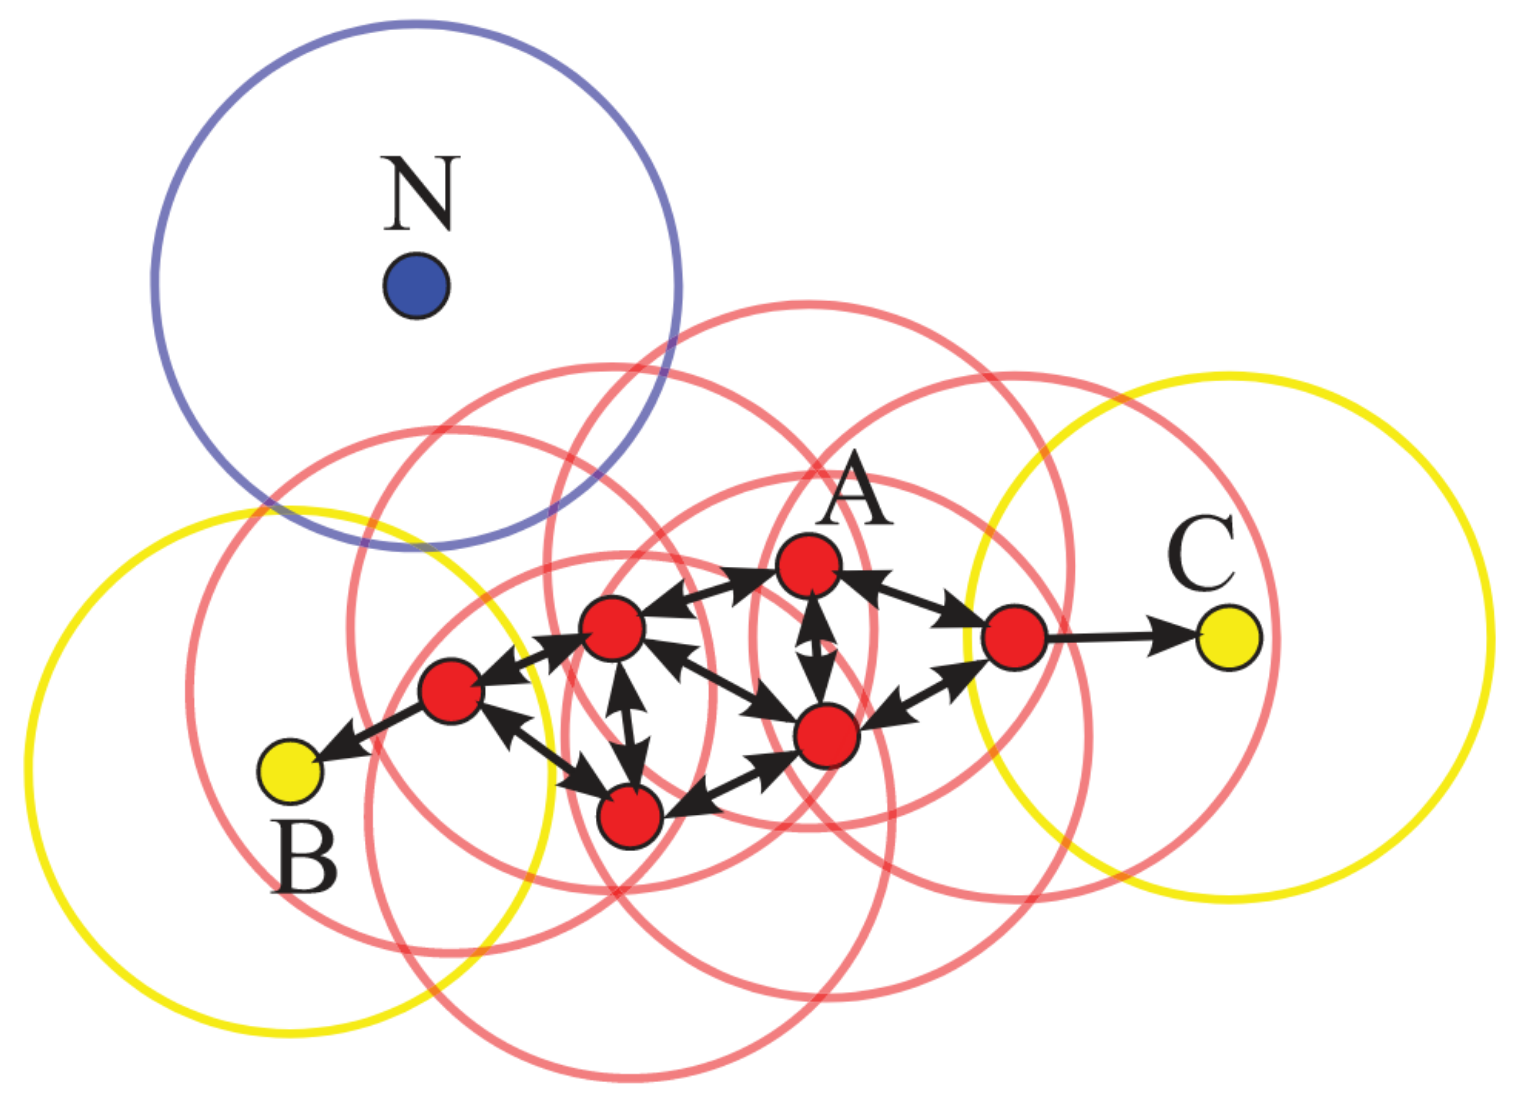
\includegraphics[width=0.5\linewidth]{obrazky-figures/dbscan}
		\caption{Illustration of DBSCAN cluster model}
		\label{dbscan_ilustration}
	\end{figure}

	Figure \ref{dbscan_ilustration} illustrates the model DBSCAN.
	Following parameters are defined:
	\begin{itemize}
			\item minPts is 4, and
			\item $epsilon$ is indicated by circles
	\end{itemize}

	In this picture you can see multiple points and four of them named A, B, C, N.
	Arrows indicate direct density reachability. Points A, B, C are density connected and B, C points are border points.
	N is not density reachable (it is not in any $\epsilon$ radius). Any point as N is considered as noise point.

	The abstracted algorithm is:\nopagebreak
	\begin{enumerate}
			\item Find neighbors in $\epsilon$ radius of every point, and find core
			points with more that minimum neigthnours (minPts).
			\item Find connected core points on the graph and merge them into clusters.
			\item Assign every non-core point to a core point. If the non-core point
			is in $\epsilon$ radius of that core-point else assign it to noise.
	\end{enumerate}

	The whole algorithm is:\todo{rewrite it and add output}
	\nopagebreak
	\begin{figure}[H]
		\centering
		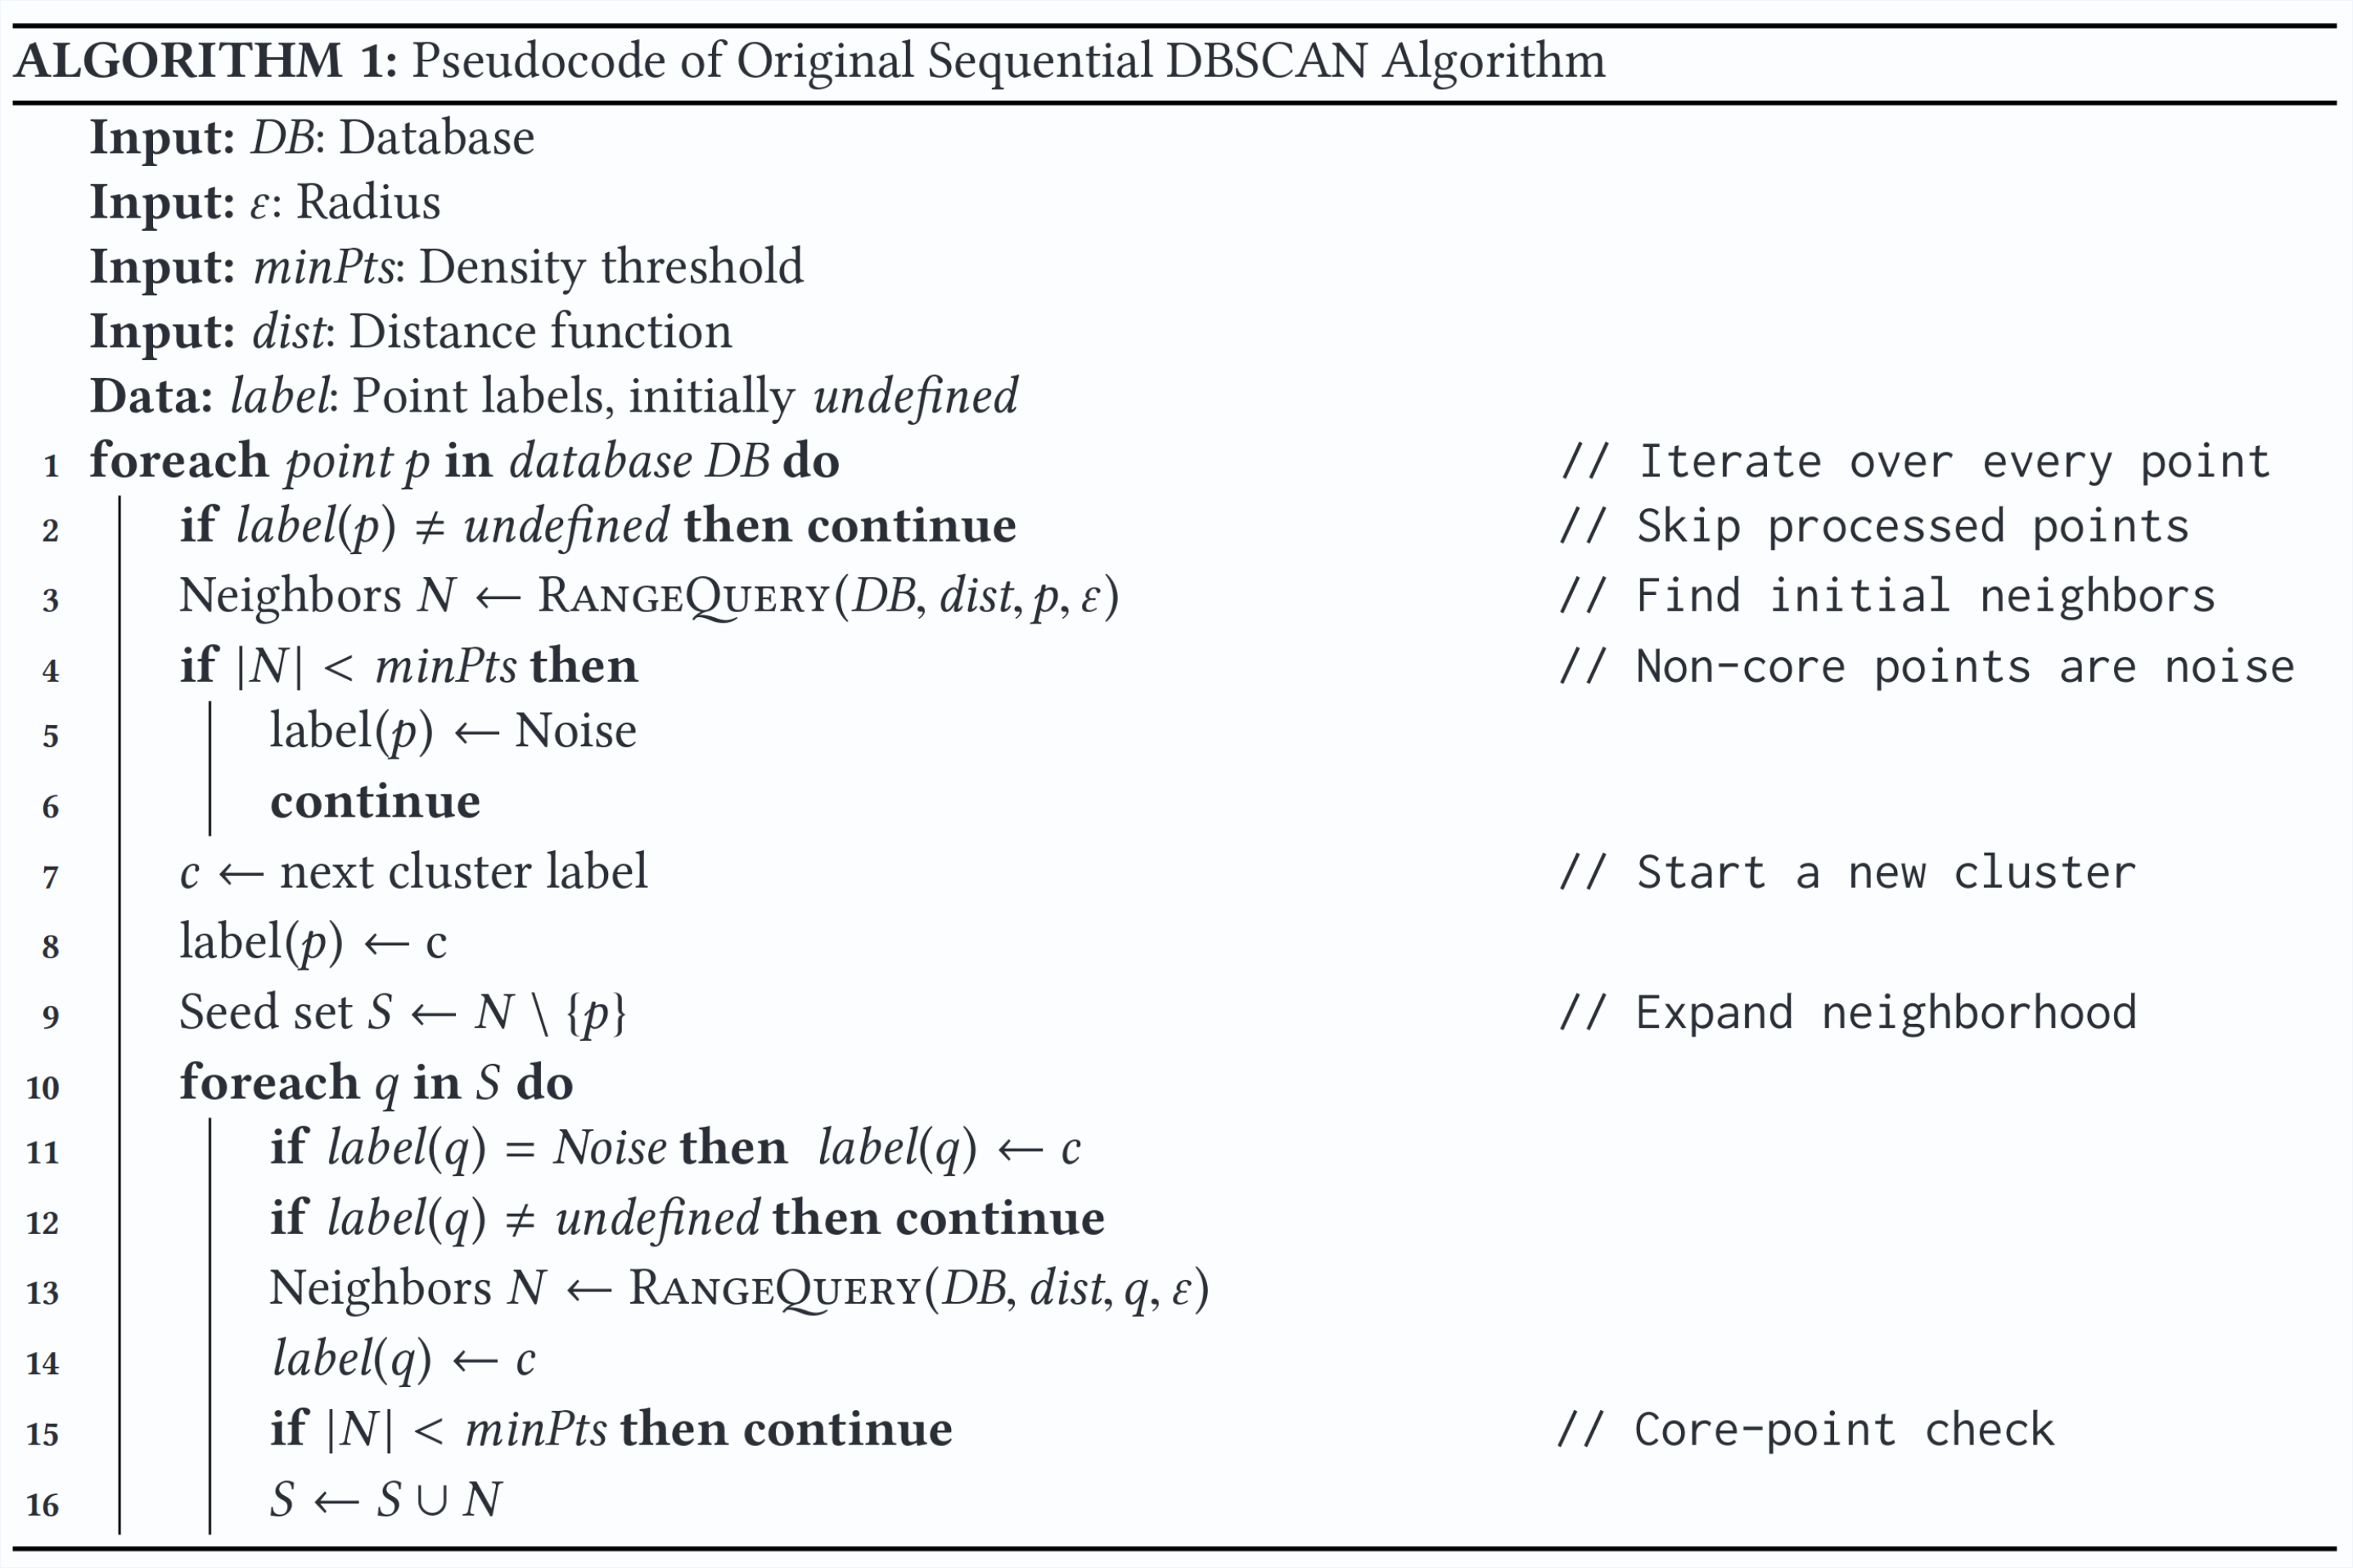
\includegraphics[width=\linewidth]{obrazky-figures/algo_dbscan}
		\caption{Illustration of DBSCAN cluster model}
		\label{dbscan_ilustration}
	\end{figure}


\subsection{Pitfalls of Clustering}
The clustering of the arguments of system call has some pitfalls.
Some of them are described bellow.

\paragraph{Address space layout randomization.}
ASLR was introduced in 2001 by Page EXec (PaX) team to defense over buffer
overflow attack, \cite{ASLR:PAX, Ganz2017}. The goal of ASLR is to provide
randomness into address space of a given task. This will add another layer of
protection against exploits which uses buffer overflow to change behavior of
attacked software.

The idea behind ASLR is that the memory segments (stack, heap, libraries, ...)
are located on different offsets during the runtime. With this technique you can
achieve that exploits can not know where exactly is located, e.g., a stack
segment in the memory. When ASLR is enabled, the analysis of the addresess in
a system call make no sense. You can not know on which offset any segment will be.

ASLR is by now implemented in many modern OS (MS Windows, GNU/Linux, NetBSD, OpenBSD, MacOS).
In Linux, this feature is enabled by a kernel. You can get information if ASLR is enabled in file e.g.:
\begin{center}
	\texttt{cat /proc/sys/kernel/randomize\_va\_space}
\end{center}

Value description:
\begin{itemize}
	\item \textbf{0} ASLR is turned off,
	\item \textbf{1} ASLR is enabled only for Shared libraries,  mmap(), VDSO, stack and heap,
	\item \textbf{2} ASLR is fully enabled.
\end{itemize}


\paragraph{String represented in memory}
The strings are represented in memory as an offset where the string
begins and ends with null termination. \cite{ISO9899} \todo{TODO cite}
For this reason seccomp can not operate with strings and we will skip string arguments as well.

\section{Parsing Expression Grammar}
Parsing expression grammar was introduced by Ford in 2004. \cite{Ford:PEG}
PEG is a type of analytic formal grammar which describes a formal language in terms of a set of rules for recognizing strings in the language.
This type of grammar is really similar to a top-down parsing languages.
As well it looks very similar to context-free grammars.

Parser that parses the PEG is named a packrat parser.
Packrat parser can be easily constructed for any language described by an LL($k$) or LR($k$) grammar, as well as for many languages that require unlimited lookahead and therefore are not LR.
Packrat parsers are also much simpler to construct than bottom-up LR parsers, making it practical to build them by hand.
It can directly and efficiently implement common disambiguation rules such as \textit{longest-match}, \textit{followed-by}, and \textit{not-followed-by}, which are difficult to express unambiguously in a context-free grammar or implement in conventional linear-time.
Finally, both lexical and hierarchical analysis can be seamlessly integrated into a single unified packrat parser.

The main disadvantage of packrat parsing is memory consumption.
The worst case asymptotic computational complexity is very similar to the conventional algorithms (linear in the size of the input).

The one of the many problems with right to left parsing algorithm is that it computes many results that are never needed.
Other inconvenience is that we must carefully determine the order in which the results for a particular column are computed.
\textit{Packrat parsing} is a lazy derivation of a tabular algorithm that solves both of these problems.
It computes results only when they are needed, in the same order as the original recursive descent parser would.


\begin{table}[h]
	\begin{center}
  \begin{tabular}{lcl}
      Addition       & $\leftarrow$ & Multiplication '+' Addition | Multiplication \\
      Multiplication & $\leftarrow$ & Primary '*' Multiplication | Primary     \\
      Primary        & $\leftarrow$ & '(' Addition ')' | Number          \\
      Number        & $\leftarrow$ & '0' | \ldots | '9'
  \end{tabular}
  \end{center}
  \caption{Example of a grammar for a trivial language}
  \label{fig:pegtl:example}
\end{table}



% \section{Translator}
% This part is responsible for translation of IDS output to libseccomp.



\chapter{Development of strace2seccomp}
%code should be using libseccomp to be secure.
%test it with some fuzzer

\section{Input}
As I mentioned earlier strace tool was chosen because it is easy to use system
call monitoring tool. It can monitor what observed program demanded from kernel.
With strace tool it is possible to trace child processes. The main advantage of
strace tool is that is does not need any of the source code files, program is not
compiled with extra flags or withount any library or it does not have to be
statically linked. This were the reasons why I chose the strace tool as an input
for the strace2seccomp.

The output from strace tool has to be normalized before procesing with strace2seccomp.
The normalization is done by providing a few runtime arguments to the strace tool.
Example:

\texttt{\$ strace -s 0 -xx -o dataset -ff nautilus }
\\
I would like to describe what they are doing in the first place.\cite{strace_man}

\paragraph{-s} is a string size. We are setting a string size to zero because
the libseccomp does not have the ability to work with strings. It does not know
how long is the string or if it is really a string. By this option the filenames
are not affected. They are printed in full length.

\paragraph{-xx} this option will switch the format of strings to a hexadecimal format.
It is much easier to parse strings in this format. It affects the filename as well.
This option is used because sometimes a non ASCII (UTF--8) character can occure in filename.

\paragraph{-f} traces children processes.

\paragraph{-o} is used for specifying the output file.

\paragraph{-ff} is helpfull when you are tracing a multiprocess program. In this
case it will create a multiple files in format NAME.PID where NAME is a provided
filename in option \texttt{-o} and PID is a process id.

\section{Class Hierarchy}
This section provides information about class hierarchy in this project.

At the beginning is the \texttt{Params} class as we can see in Figure
\ref{fig:class:params}. In constructor of \texttt{Params} class is executed
getopt library to acquire a runtime arguments. The omitted arguments are then
saved in class variables. By this variables the whole tool is instrumented.

\begin{figure}[h]
	\centering
	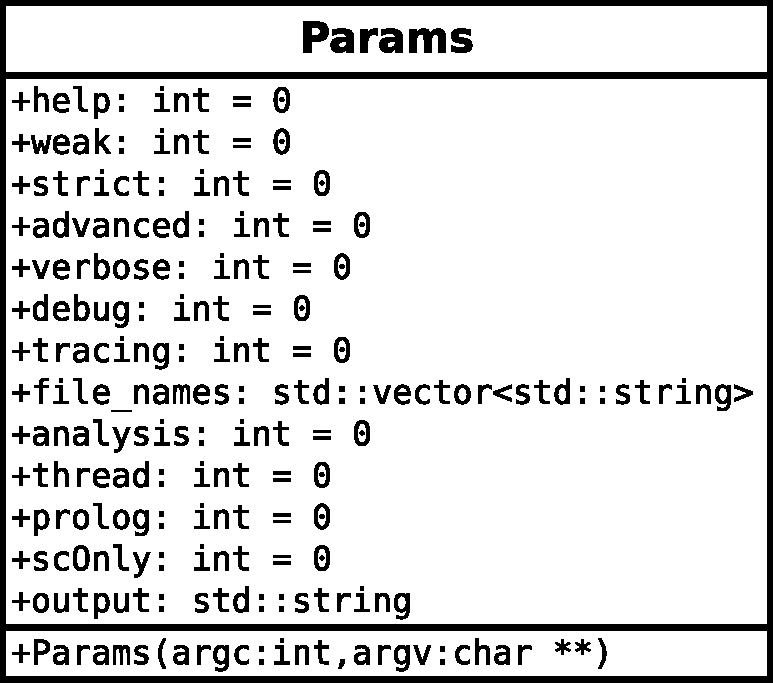
\includegraphics[width=0.35\linewidth]{obrazky-figures/class/params.pdf}
	\caption{Class diagram that shows representation of runtime arguments}
	\label{fig:class:params}
\end{figure}

The next class diagram in Figure \ref{fig:class:ids} show us an Intermediate
Data Structure (IDS). The IDS is handled with multiple components in this
project, i.e., parser saves information there, etc., description is in Section
\ref{ids:description}. As you can see the \texttt{\_argument\_t} class has three
constructors.  Here could be used design pattern factory however there are only
two different cases of creating an object so it was not needed. The
\texttt{\_argument\_t} class contains individual data about argument, e.g., the
format value says if the argument is in 'key=value' or 'value' form. The actual
value is stored in container \texttt{std::variant}. This is the C++17 equivalent
of enumeration in C language.

\texttt{Syscall\_t} class in Figure \ref{fig:class:ids} is dependant  on the
\texttt{\_argument\_t}. This class contains information about syscall, e.g.,
name, number of arguments, and actual arguments. In this class is defined
\texttt{print()} method that can print structurised data from syscall.

\begin{figure}[h]
	\centering
	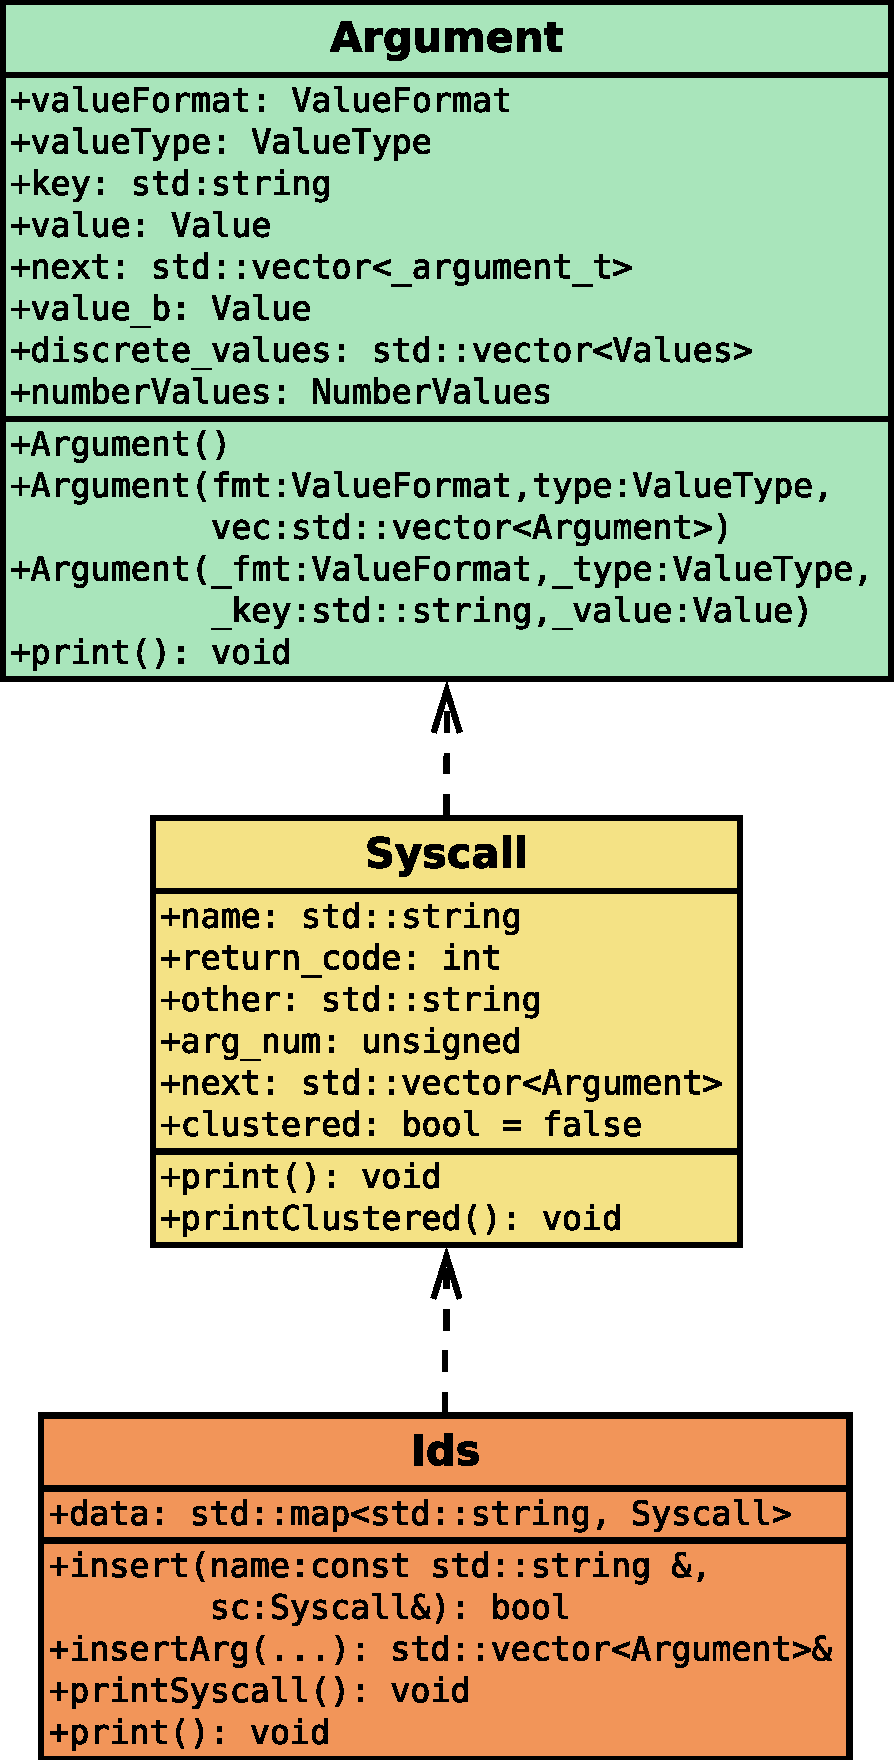
\includegraphics[width=\linewidth]{obrazky-figures/class/arg_sc.pdf}
	\caption{IDS representation in class diagram}
	\label{fig:class:ids}
\end{figure}

\begin{figure}[h]
	\centering
	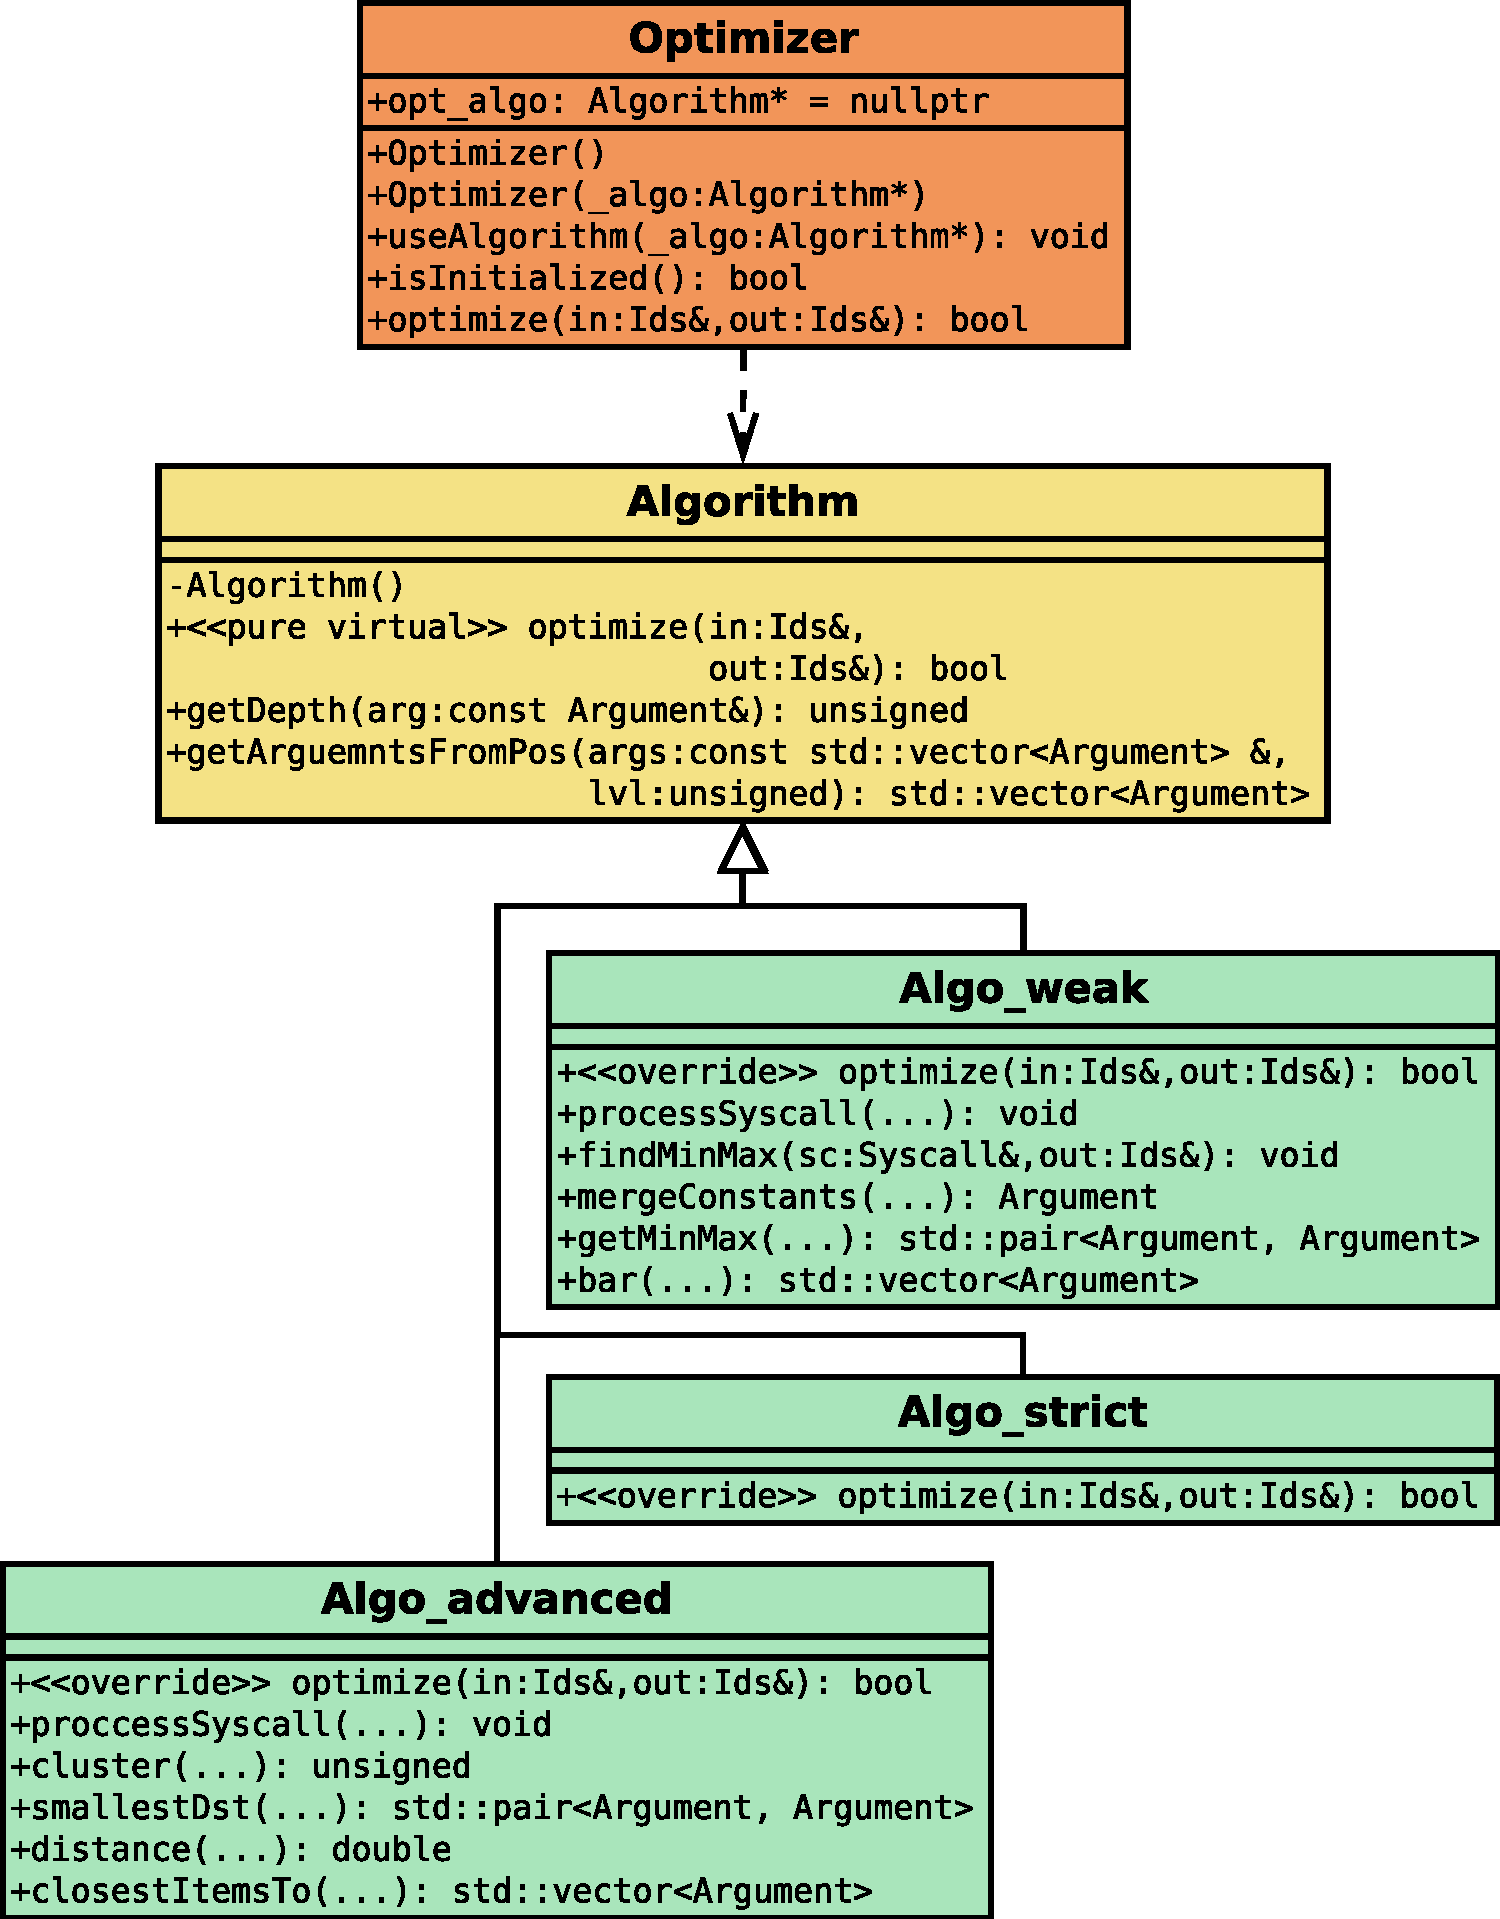
\includegraphics[width=\linewidth]{obrazky-figures/class/algo.pdf}
	\caption{algorithms}
	\label{fig:class:algo}
\end{figure}

\begin{figure}[h]
	\centering
	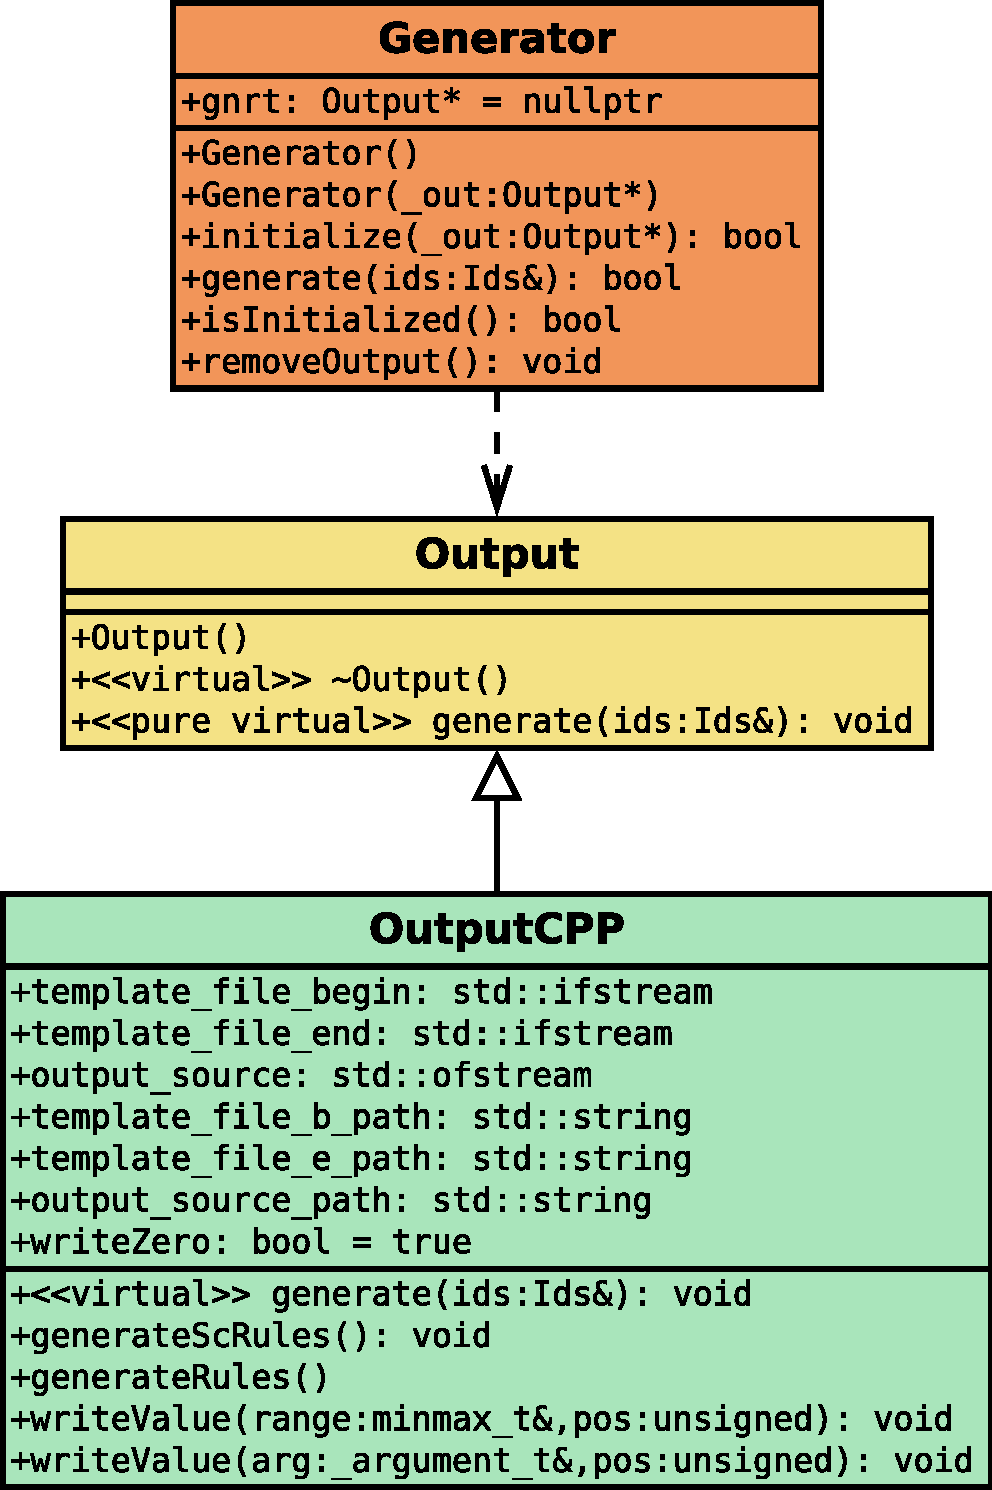
\includegraphics[width=0.6\linewidth]{obrazky-figures/class/output.pdf}
	\caption{output}
	\label{fig:class:output}
\end{figure}

\section{Output}
The strace2seccomp tool is generating a source code for C/C++.
In the source code is used seccomp library to provide system call blocking.
The example of a generated source code is in Appendix \ref{lst:example1}

\section{Used software}
In this section, I want to mention which software I used to develop a strace2seccomp tool.
Firstly, I mention compilers used in this project and after that valuable tools for developments.

\subsection{Compilers}
\label{subsec:compilers}
In this project, I used two compilers. The reason is simple.
Every compiler can detect a different set of errors and warnings during the compilation.
And at the time of doing project one of the reason of compiling with two compilers
was to compare the execution times with optimizations turned on.

In the project, \texttt{libc++} and \texttt{libc++ ABI} from LLVM project was
used. The reason for using implementation from LLVM project was that in the GNU
implementation, there was a bug which affected a C++17
functionality\footnote{\url{https://bugs.debian.org/cgi-bin/bugreport.cgi?bug=877838}}.

\paragraph{GNU Compiler Collection.}GNU Compiler Collection is a part of the GNU project.
It aims to improve compiler used in the GNU ecosystem.
GCC\footnote{\url{https://gcc.gnu.org/}} uses an open development environment.
It includes front ends for C, C++, Objective-C, Go etc.
as well as libraries for these languages. It was firstly written for GNU operating system\footnote{\url{https://www.gnu.org/gnu/thegnuproject.html}}.
The compiler collection is released under the GPL license, other components, e.g., as runtime libraries are distributed under various free licenses.

\paragraph{LLVM/Clang.}
The goal of Clang\footnote{\url{https://clang.llvm.org/}} project is to provide a new C based language front-end (C, C++, Objective-C,) for the LLVM\footnote{\url{http://www.llvm.org/}} compiler.
It is released under NCSA Open Source Licence. Clang is designed to be highly compatible with GCC.
It supports most of the GCC compilation flags and unofficial language extensions\footnote{\url{https://clang.llvm.org/docs/LanguageExtensions.html}}.
\todo{maybe mention error logs}


\subsection{Dynamic and Static Code Analysis}
For correct development is necessary to find as many bugs as possible during the this phase.
This goal was achieved by ussing dynamic and static analysis tools.
For static analysis was used an LLVM project named clang-tidy and for

\paragraph{LLVM/Clang-tidy.}
Clang-tidy is a clang-based ''linter'' tool\footnote{\url{http://clang.llvm.org/extra/clang-tidy/}}.
Its purpose is to diagnose and fix typical programming errors,
like interface misuse, style violation, or bugs that can be deduced via static analysis.
Clang-tidy diagnostics are designed to assert code that has invalid coding standard or is otherwise problematic.
It has options to diasable some false positive warnings (e.g. \texttt{\textbackslash\textbackslash NOLINT}).

\paragraph{AddressSanitizer.}
AddressSanitizer\footnote{\url{https://github.com/google/sanitizers/wiki/AddressSanitizer}} (ASan) is a memory error detector for C/C++ developed by Google.
ASan is very fast and the average slowdown of the instrumented program is \textasciitilde 2x.
The tool consists of a runtime library which replaces the \texttt{malloc} function and compiler module (currently as LLVM pass).
The tool supports multiple architectures, e.g., x86, x86\_64, ARM, ARM\_64, MIPS, PowerPC64, etc.
It is part of the both compilers mentioned above in Subsection \ref{subsec:compilers}.

Usage of ASan is very straightforward. You have to only add compiler arguments:\\
\begin{center}
	\texttt{-fsanitize=address -fno-omit-frame-pointer}
\end{center}
The first parameter turns on the ASan and the second one prints a nicer stack trace in error messages.
It is adviced by developers to use optimization, e.g., \texttt{-O1}, to get reasonable performance.

\subsection{Others}
asdf
\paragraph{Git}
Git\footnote{\url{https://git-scm.com/about}} is a source code manager (SCM). It stands out of the group of SCMs by its branching model.
Git allows and encourage you to have multiple local or remote branches that can be entirely independent.
This provides features like:
\begin{itemize}
	\item Context Switching
	\item Feature Based Workflow
	\item Role-based Codelines
	\item Disposable Experimentation
\end{itemize}
Other benefit of Git is that it does nearly all operations locally.
This gives the tool huge speed advantage.
Git was built to work with Linux kernel, that means it can effectively handle large repositories.
The st2se used repository hosting on GitHub.

\paragraph{Artistic Style}
Astyle\footnote{\url{http://astyle.sourceforge.net/}} is a source code formatter and beautifuller.
Works with C, C++ Objective-C, C\# and Java programming languages.
The motivation to use this tool is to have uniform code style.
Some of the editors by default insert spaces instead of tabs when pressing a key.
Other editors have the abillity to insert space before tab lines to ''pretty up'' the code (Emacs).
The solution to this problem is to use Artistic Style formatter.
It can normalise the source code by rules defined in a configuration file provided by a developer of the project.

\paragraph{LCOV and GCOV}
LCOV\footnote{\url{http://ltp.sourceforge.net/coverage/lcov.php}} is an extension to GCOV, a GNU tool which can determine what parts of a program was executed while running particular testcase.
It can provide information about how many times that part of program was executed.
LCOV implements to GCOV following additional functionality:
\begin{itemize}
	\item HTML based output with coverage rates indicated by specific color, i.e., green is 100\% and red is 0\% coverage.
	\item Support for large projects. It allows you to browse over overview pages that shows coverage data
	by providing: a directory view, a file view and a source code view.
\end{itemize}
LCOV was designed like Git to support Linux kernel, but works as well on standard user space applications.
This tool uses line coverage technique and it is the poorest coverage from the coverage types point of view.


\section{Usage}
How to run the st2se tool



\chapter{Software Verification}
This chapter will describe activities used to assure quality control of the developed tool.
First, I want to introduce on which aspects we will focus.
One of the aspects is \textit{module testing}.
The main purpose of module testing is to detect errors in submodules, in communication among them, in passing data through data structures.
Another aspect of verification is \textit{system testing} merged with \textit{acceptance testing}.
In this type of testing we will check if the strace2seccomp tool has a valid architectural design.
Next aspect which will be checked is \textit{static analysis}.
Static analysis is type of testing which does not require to run the program but requires a source code of the tool.
The static analyzer will analyse the source codes with different heuristics and produces an analysis of detected errors. % cite ITS lectures.


\section{Module Testing}
Module testing is part of whole quality control process.
This testing can provide us how functional are particular components and if they meet the requirements.
Table \ref{table:moduletesting} shows us the description of module's test suits.

\begin{table}[h]
	\centering
	\begin{tabular}{|l|p{10cm}|}
		\hline
		\textbf{Module / Component}	&	\textbf{Test descriptiom} \\ \hline \hline
		Params 											& Validity of recognized runtime arguments \\ \hline
		StraceParser								& Syntax testing, validity of parsed data, correct error handling \\ \hline
		Algorithm 									& Testing correctness of algorithms \\ \hline
		Output                      & Check the validity of generated policy \\ \hline
	\end{tabular}
	\caption{Test plan}
	\label{table:moduletesting}
\end{table}

\subsection{Params Testing}
about using params class in custom test set and manualy check if the correct flags was ommited.

\subsection{StraceParser Testing}
StraceParser module is responsible for parsing the strace output and translates it to intermediate data structure.
Testing of this module can be done with various techniques.
First one which is used is fuzzy testing or fuzzing described in section below \ref{fuzzing}.

\subsubsection{Fuzzing}
\label{fuzzing}
The term fuzzing was first used by professor Barton Miller who used fuzzing to test robustness of UNIX applications in 1989 \cite{Takanen:2008:FSS:1404500, Marhefka2013}.
Fuzzing is a testing method which generates an unexpected input on tested software and then is observing if the software crashes. The whole process is
typicaly automated or semiautomated that involves repeatedly manipulating and supplying input data to targeted program.
Some modern fuzzers (programs that generates a stochastic input), record every crash or halt of a tested program.
The stochastic data are in most cases invalid to observer how application handles invalid
states and boundary conditions.
"The name comes from modern applications tendency to fail due to random input caused by line noise on 'fuzzy' telephon lines."\cite{Takanen:2008:FSS:1404500, N2LYDLnqzEFYp0wM, takanen2009fuzzing}
In other literature fuzzing can be named by these terms:
\begin{itemize}
	\item Negative testing
	\item Syntax testing
	\item Dirty testing
	\item Rubustness testing
	\item Protocol mutation
	\item Fault injection
\end{itemize}

\noindent
Fuzzers can be divided into two large groups:

\begin{itemize}
	\item \textbf{Generation-based} fuzzers creates test suite from scratch by modeling the target grammar.
	\item \textbf{Mutation-based} fuzzers needs an (in)valid input file. The file is mutated by various techniques.
	The mutation can be e.g. bitflip, byte change, duplicate or swap some chunks in the input file.
	The mutated test case is then provided to a tested program.
\end{itemize}

For us is interresting \emph{Mutation-based} group because is easier to setup and
is more availible in open source comunity. There are many options to choose so here is
a little comparison of most popular fuzzers:

\begin{itemize}

	\item \textbf{Bunny the Fuzzer}\footnote{\url{https://code.google.com/archive/p/bunny-the-fuzzer/}} is a closed loop, general purpose fuzzer for C programs.
	The fuzzer uses compiler-level integration which means that it injects reliable instrumentation hooks into an object file.
	Those hooks enable the fuzzer to trace the program, and can provide real-time feedback. This architecture provides a possibility
	to considerably improve coverage of testing process. The injection of the hooks
	needs to be done by the compiler scripts.
	This fuzzer  subset of American Fuzzy Lop. This project is now deprecated.

	\item \textbf{American Fuzzy Lop}\footnote{\url{http://lcamtuf.coredump.cx/afl/}}
	is a security oriented fuzzer that add compile-time instrumentation. It is
	supperset to really similar Bunny the Fuzzer. The fuzzer has implemented many
	researched fuzzing capabilities (bit / byte flips,  simple arithmetics, known
	integers, test case splicing, \ldots). Compared to other instrumented fuzzers it
	has moderate overhead and as little configuration as possible. The disadvantage
	of the tool is that it needs to be executed multiple times to achieve
	multiprocess or multithread fuzzing.

	\item \textbf{Honggfuzz}\footnote{\url{http://honggfuzz.com/}} us a evolutionary, security oriented, easy to use fuzzer with analysis options.
	The main advantage of this mutation based fuzzer is that it is multi-process and multi-threded without need to run multiple copies of fuzzer.
	The file corpus is automatically shared and improved among the processes / threads.
	Authors of the fuzzer says that it is ''blazing fast when it works in persistent fuzzing mode''.
	For monitoring of target (process under test) it uses low-level interface (e.g ptrace in Linux).
	It supports several hardware based (Intel BTS, Intel PT) and software based fuzzing methods.

	\item \textbf{Radamsa} is fuzzing tool\footnote{\url{https://github.com/aoh/radamsa}} developed at the Oulu university.
	The motivation for building this fuzzer was to make robustness testing accessible to independent developers.
	Existing tool were considered hard to use and to customize to fit the project.
	The fuzzer is command line tool, on input it expects multiple files (samples), and generates mutated files.
	So by the output Radamsa is considered as a mutation-based fuzzer.
	The tool includes feature aiding in automatizing test runs.
	This is achieved by specifying number of wanted test runs with unique mutated files.
	Another parameter that can be set is random seed for mutation.
	On the other hand the tool does not provide a option to monitor target (program under test).
	Radamsa is multiplatform so it is built for Windows and Linux.\cite{radamsaThesis}

	\item \textbf{Oss-fuzz} is a complex project developed by Google.\footnote{\url{https://github.com/google/oss-fuzz}}
	The architecture of this project is that the ClusterFuzz (fuzzer tools)
	automatically pulls the newest source code from repository and it will starts
	fuzzers and sanitizers \footnote{Dynamic testing tool that can detect bugs and
	faults during the execution. Typicall sanitizers are \textit{ASan},
	\textit{DFSan}, \ldots}. When some bug or fault occurs it is automaticaly
	reported to the OSS-fuzz issue tracker. Project owners are then notified with
	email about the issue. When the fix is submitted ClusterFuzz automaticaly
	verifies the fix adds a comment to issue tracker and closes the issue.

\end{itemize}


\subsubsection{Fuzzing results}
The chosen fuzzer was AFL for its ability of fast deployment and easy of use.
The opposite example is Oss-fuzz which is the whole infrastructure for fuzzing and bug hunting.

In fuzzed program was enabled only parsin every other module was turned off.
The fuzzer run straight twenty one days and during this time it was discovered
three false positive hangs and no crashes. Fuzzing run in four threads on Intel
Core i7-4810MQ. Overall was the fuzzed program executed 3,567,228,619 times.

The number of execution per second was not stable on master thread because it
was necessary to instrument other three processes. This instability can be
seen among Figures \ref{fuz:result1a}, \ref{fuz:result2a}, \ref{fuz:result3a}
and \ref{fuz:result4a}.

\todo{check the fuzzer output}

\begin{figure}[H]
	\centering
	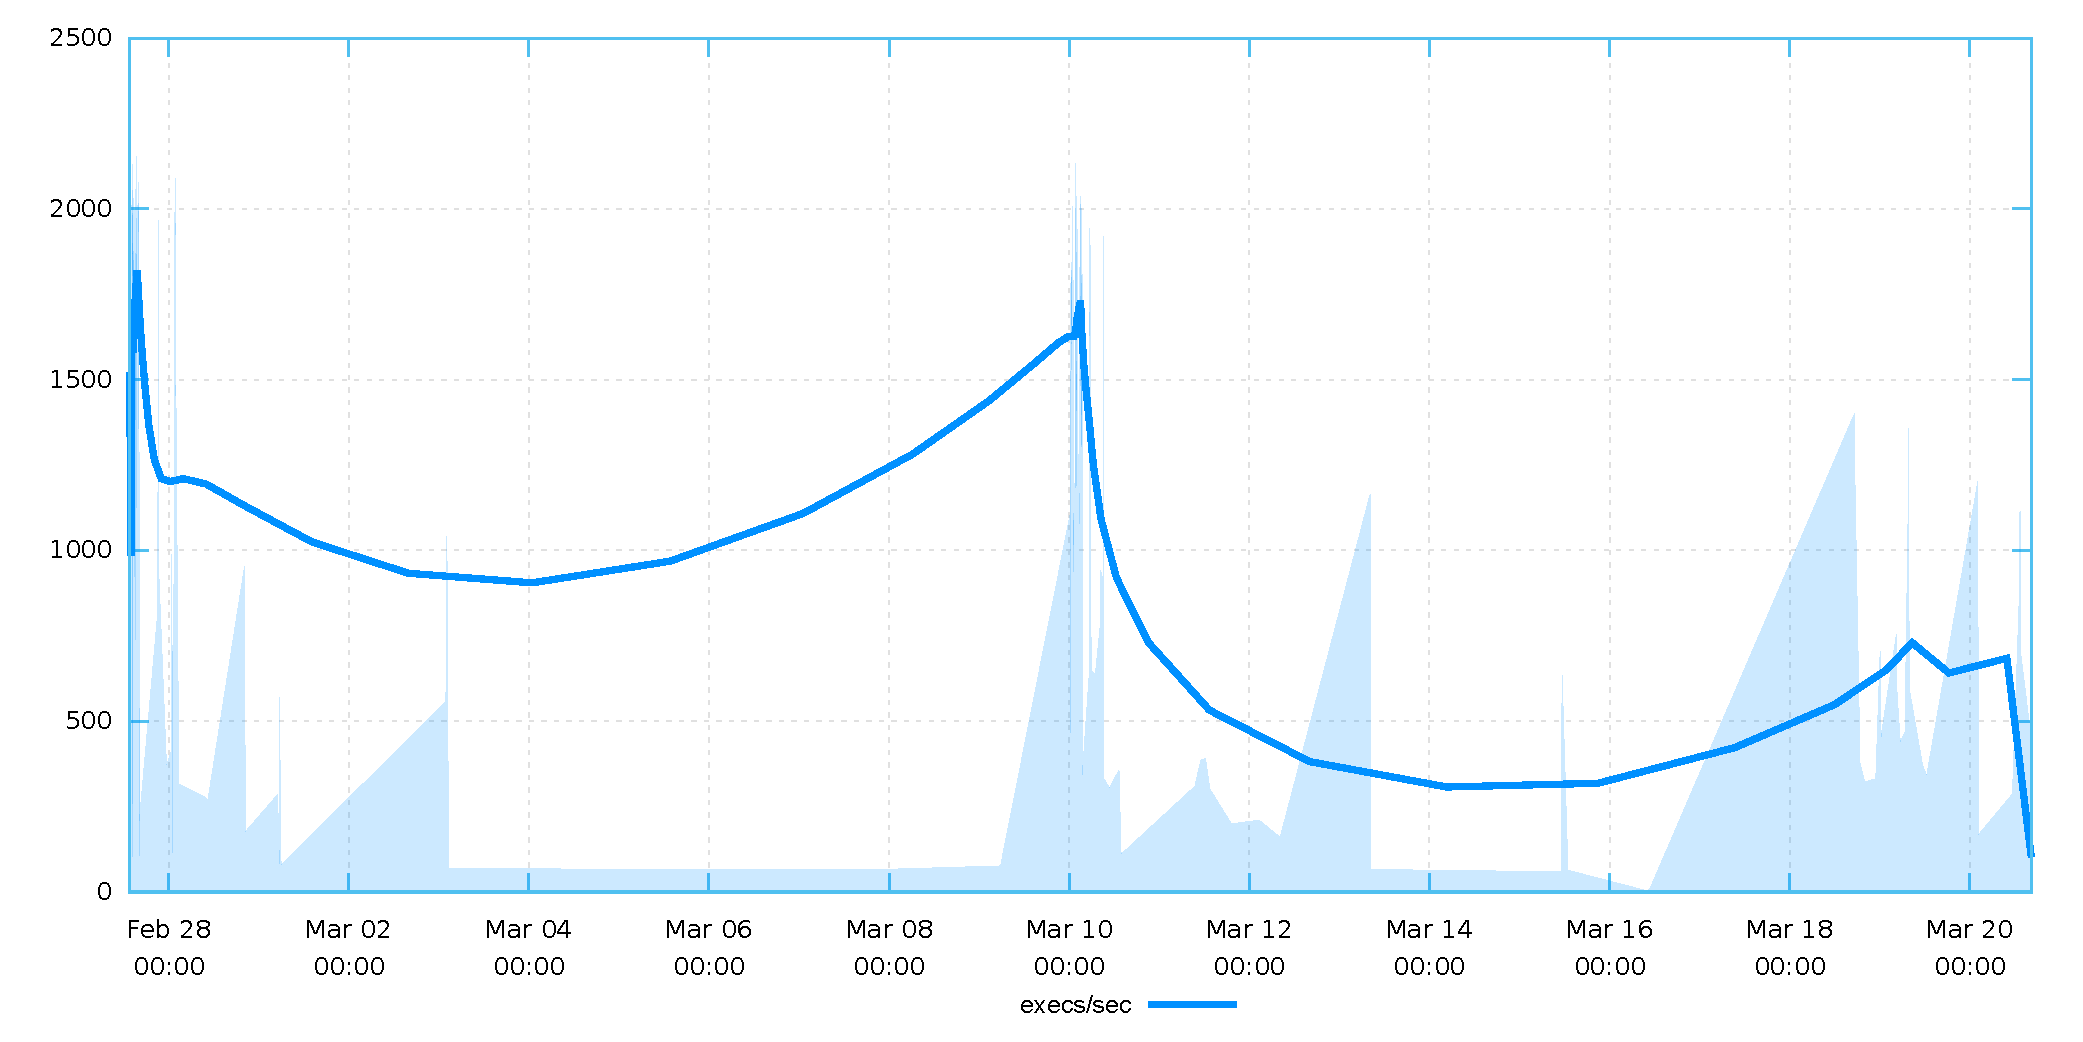
\includegraphics[width=\linewidth]{obrazky-figures/master/exec_speed.pdf}
	\caption{master/exec\_speed}
	\label{fuz:result1a}
\end{figure}

\begin{figure}[H]
	\centering
	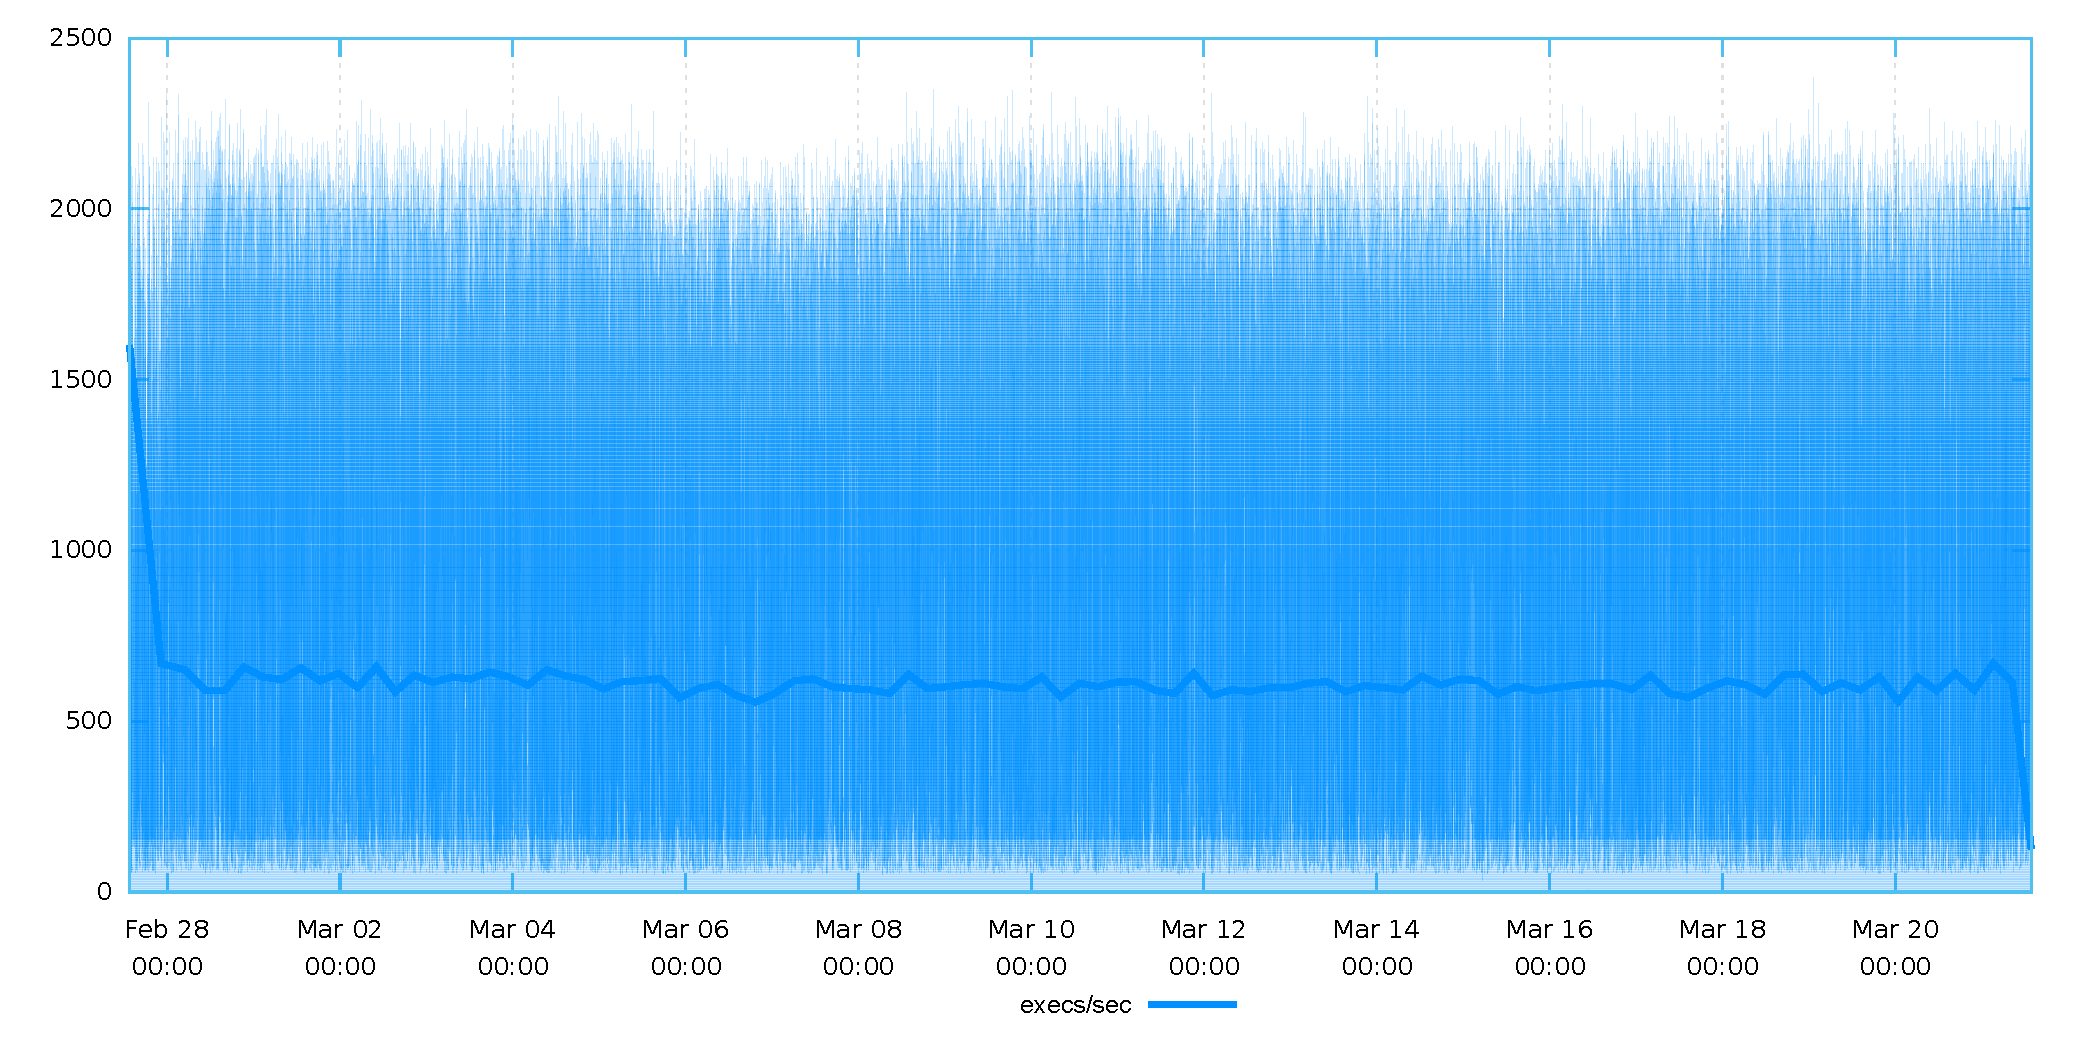
\includegraphics[width=\linewidth]{obrazky-figures/thread_1/exec_speed.pdf}
	\caption{thread\_1/exec\_speed}
	\label{fuz:result2a}
\end{figure}

\begin{figure}[H]
	\centering
	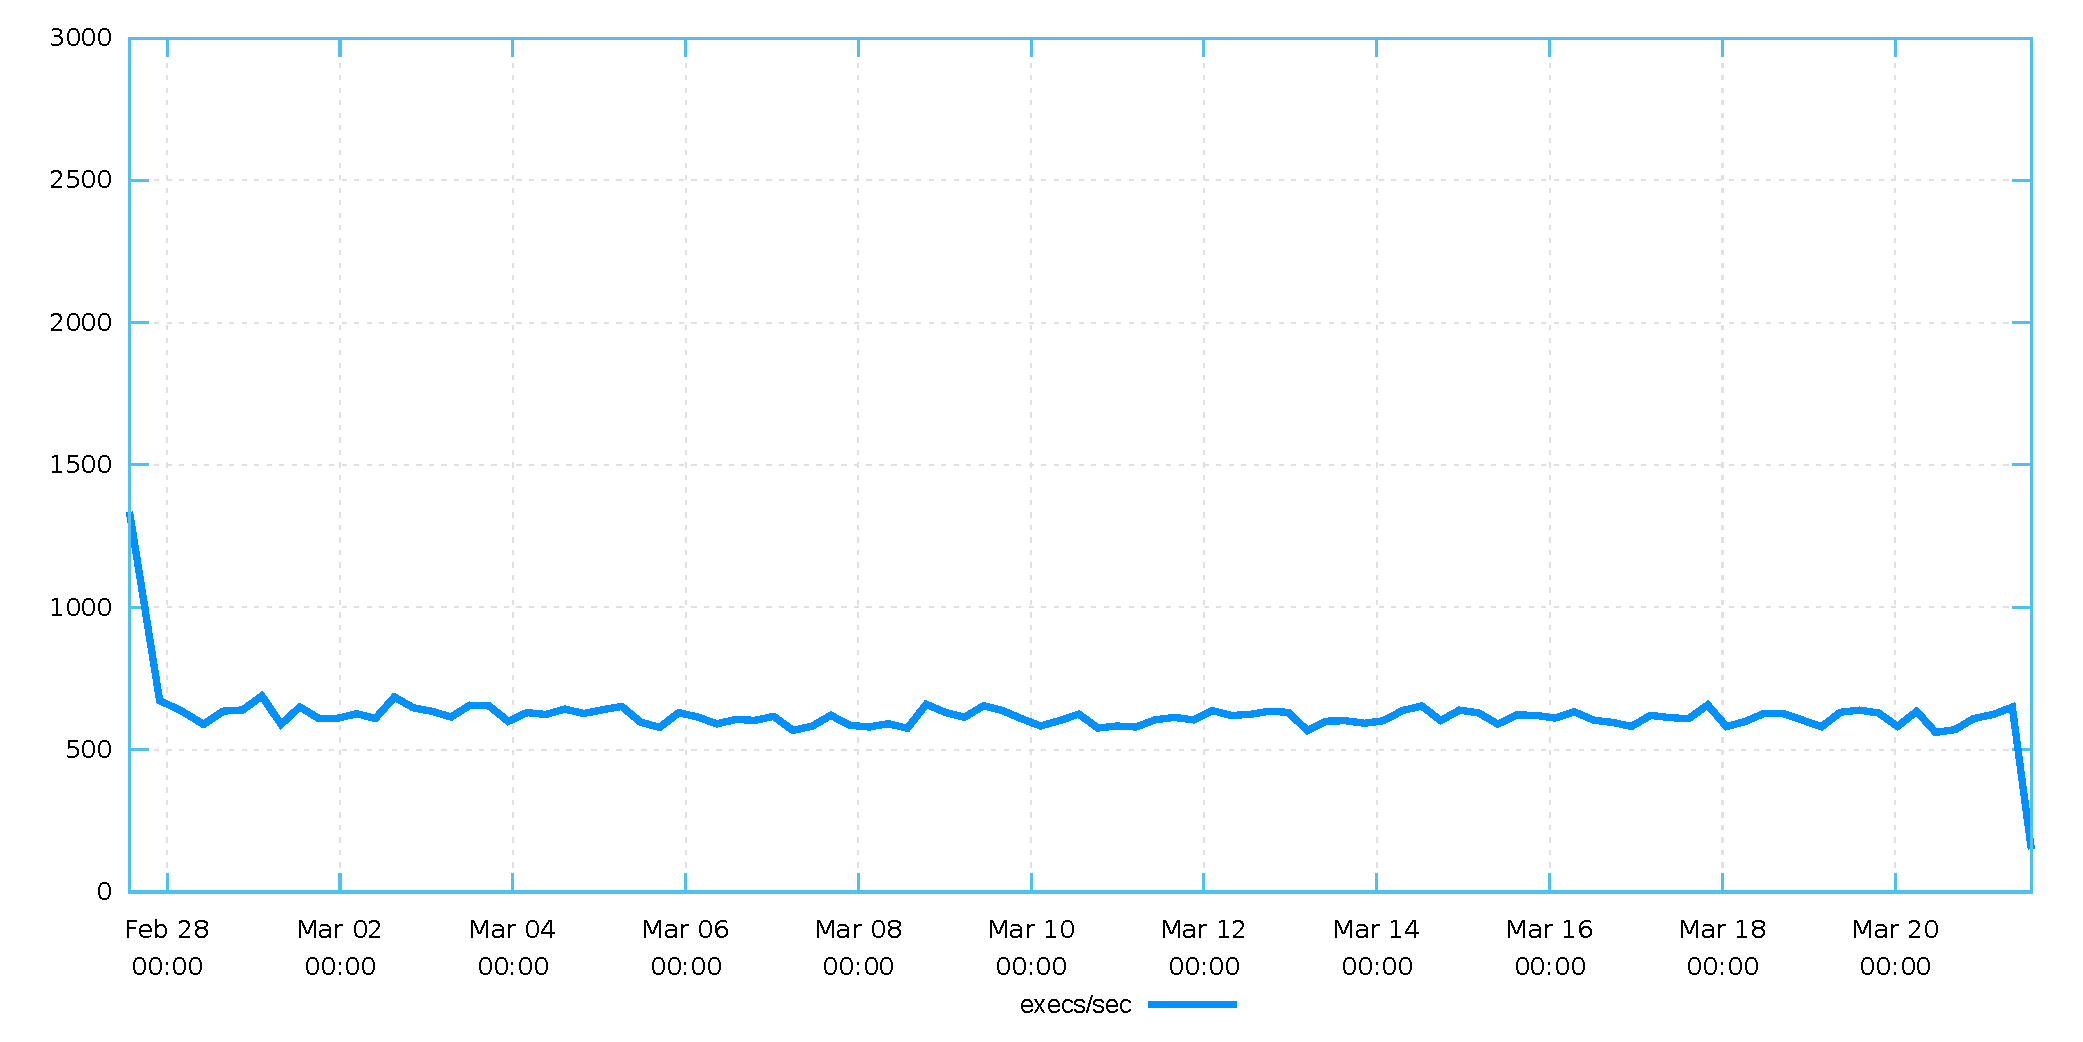
\includegraphics[width=\linewidth]{obrazky-figures/thread_2/exec_speed.pdf}
	\caption{thread\_2/exec\_speed}
	\label{fuz:result3a}
\end{figure}

\begin{figure}[H]
	\centering
	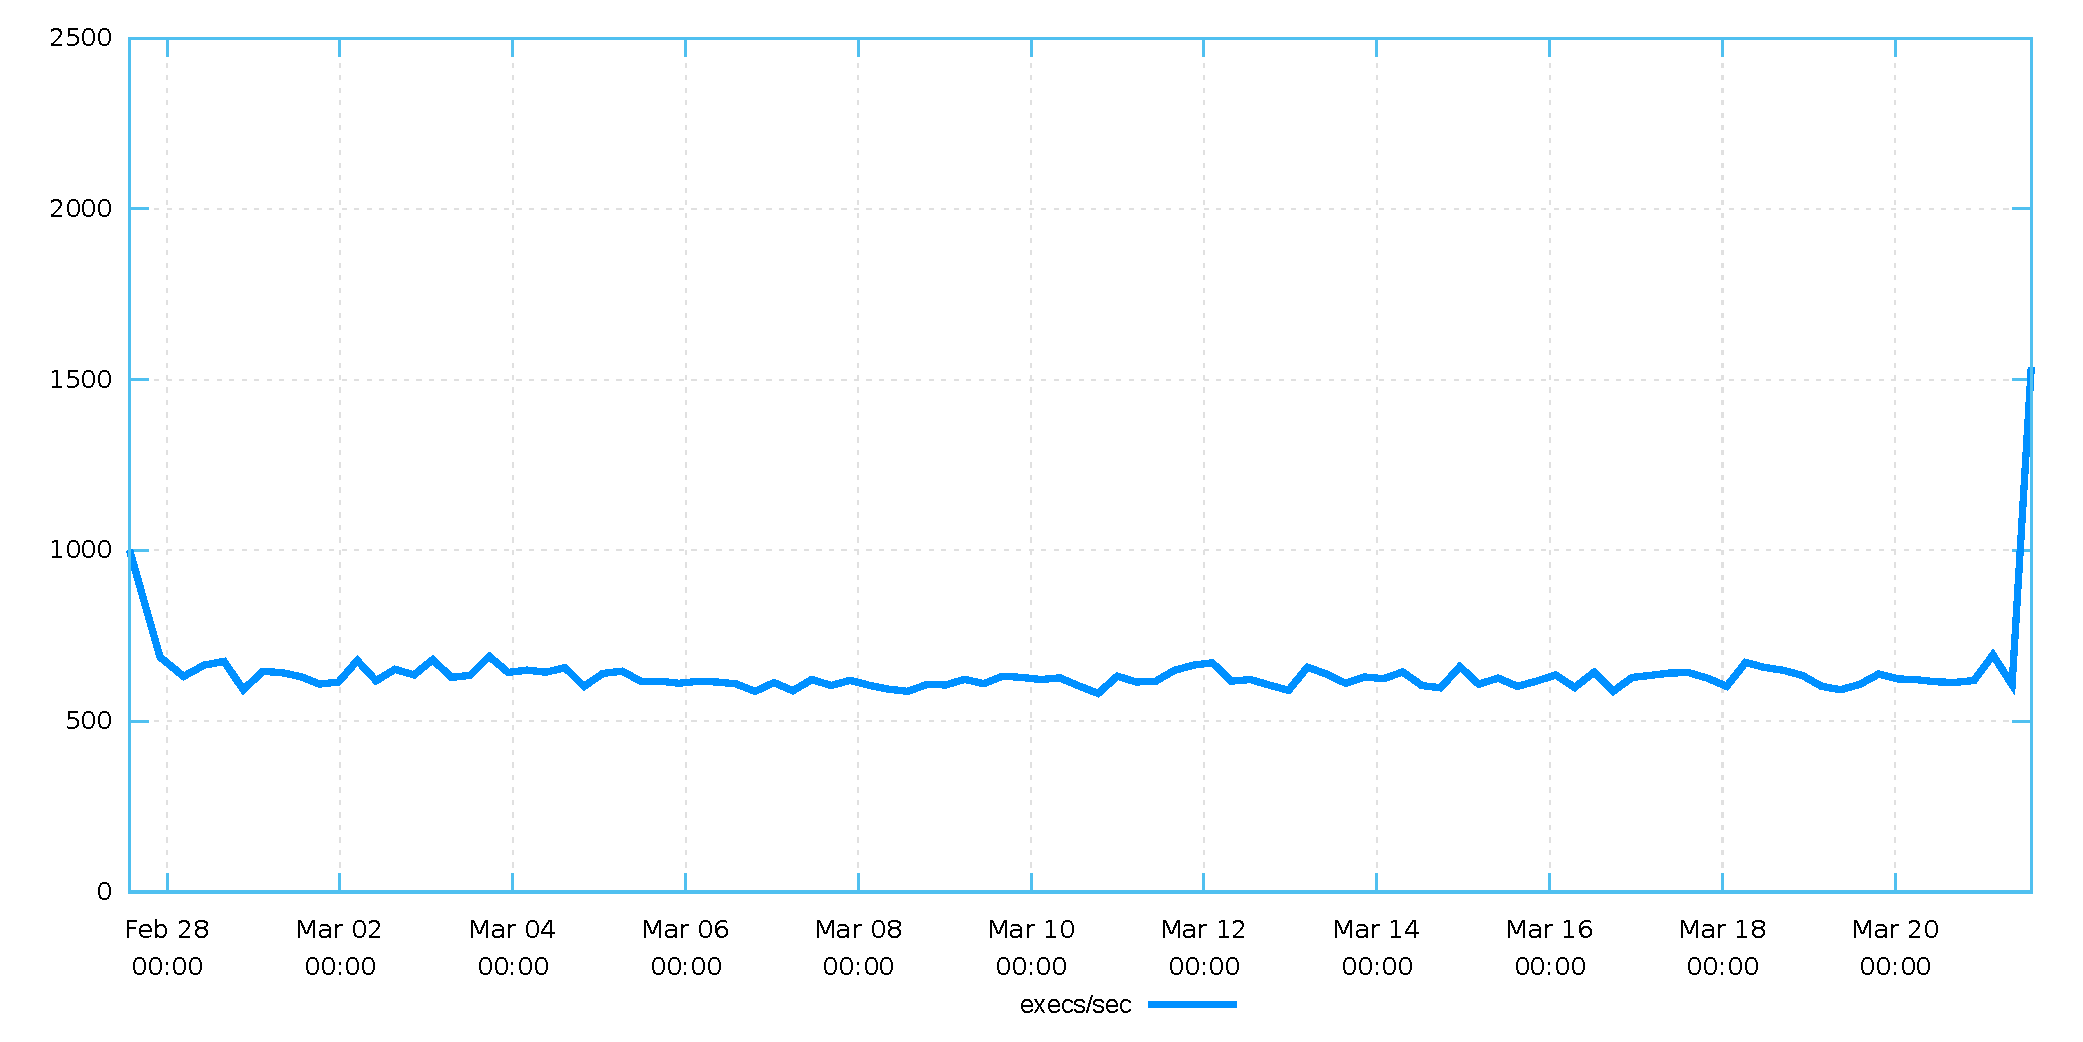
\includegraphics[width=\linewidth]{obrazky-figures/thread_3/exec_speed.pdf}
	\caption{thread\_3/exec\_speed}
	\label{fuz:result4a}
\end{figure}

asdfasdfasf
asdfasdfasf
asdfasdfasf

\begin{figure}[H]
	\centering
	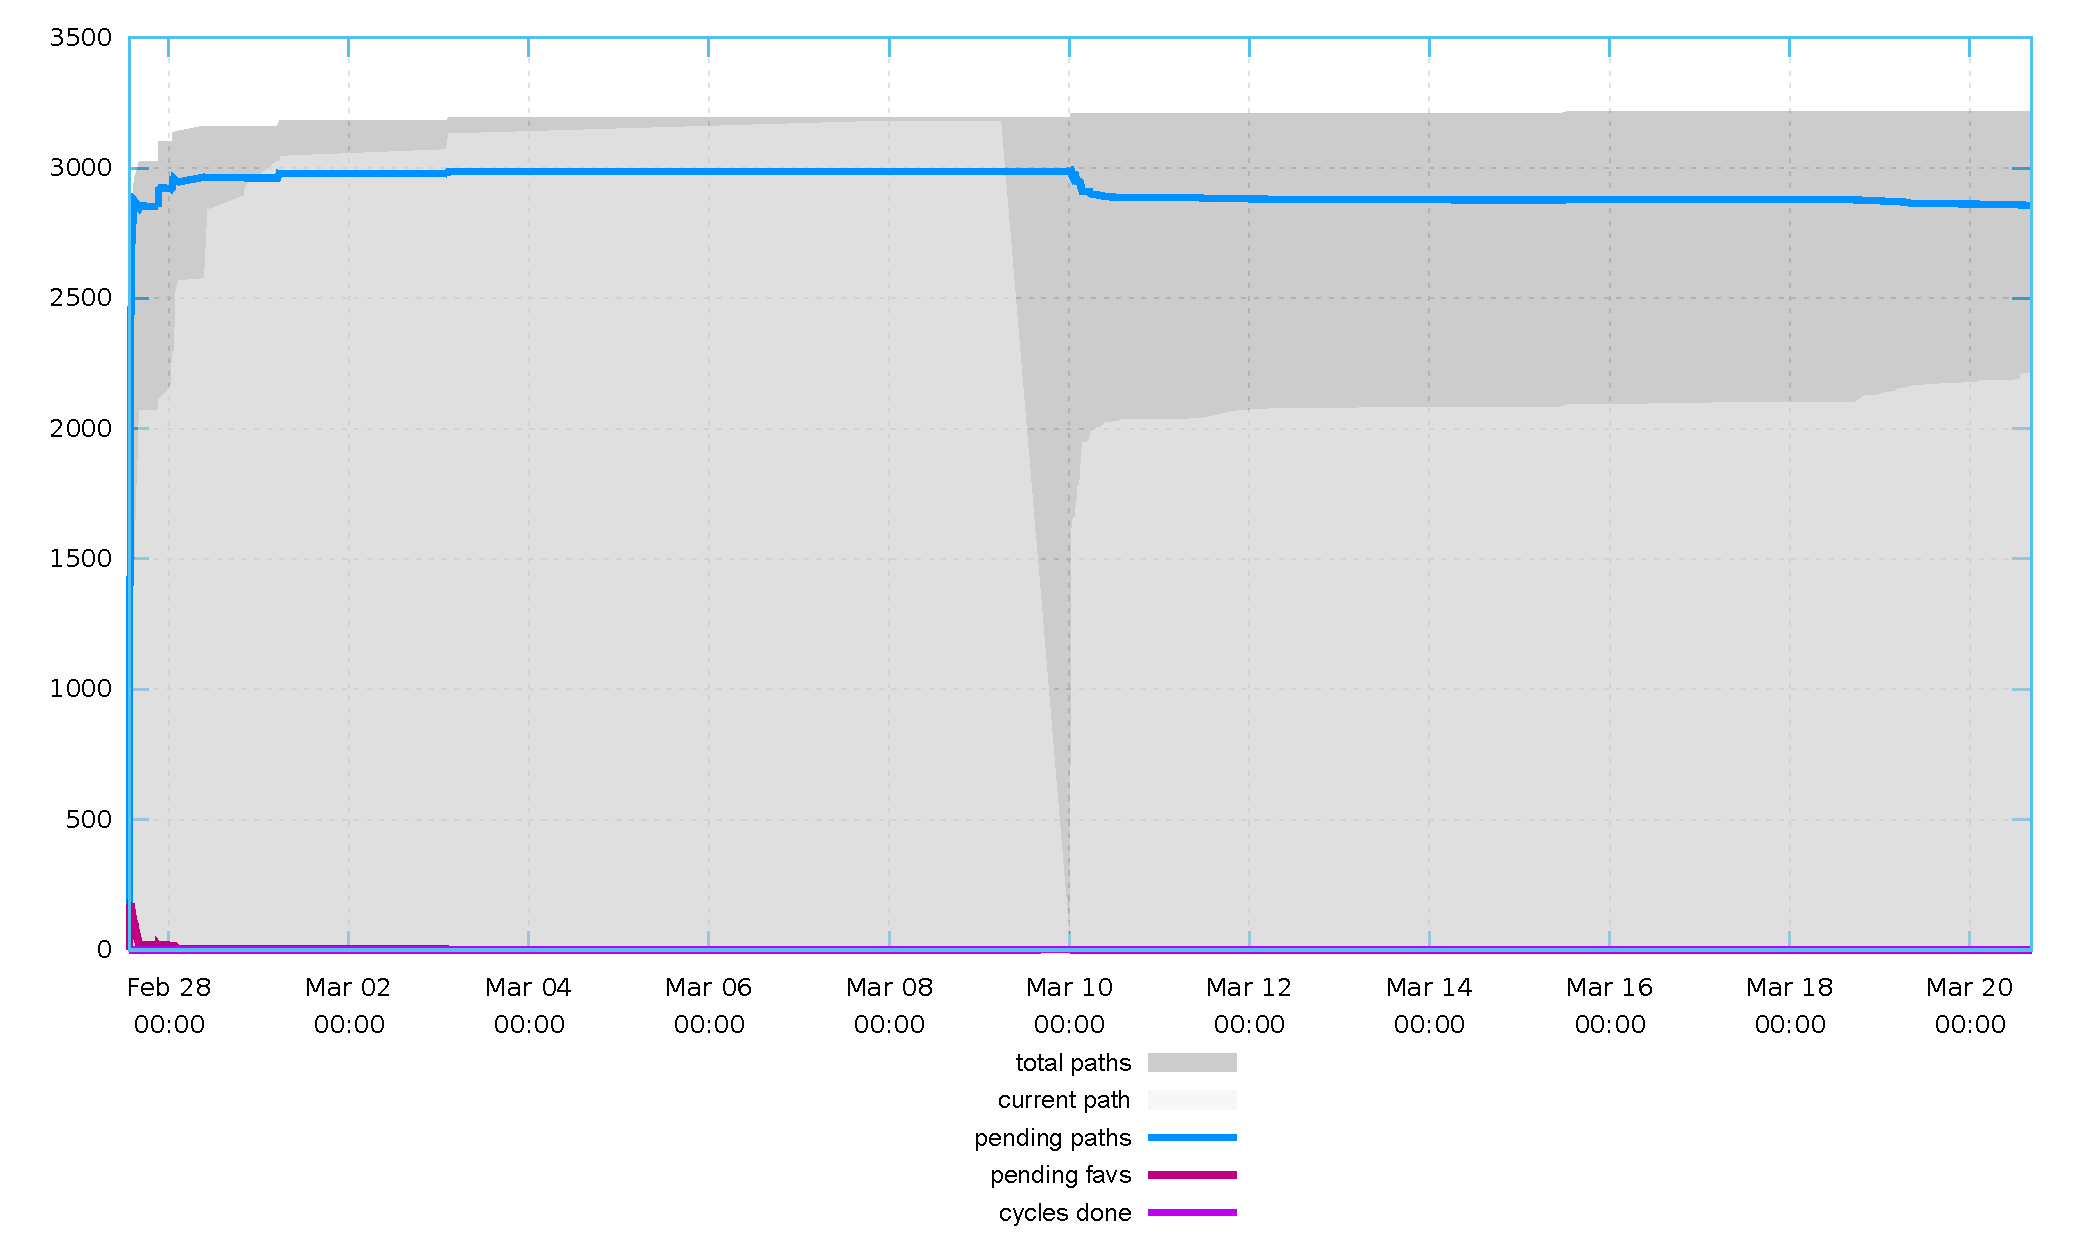
\includegraphics[width=\linewidth]{obrazky-figures/master/high_freq.pdf}
	\caption{master/high\_freq}
	\label{fuz:result1b}
\end{figure}

\begin{figure}[H]
	\centering
	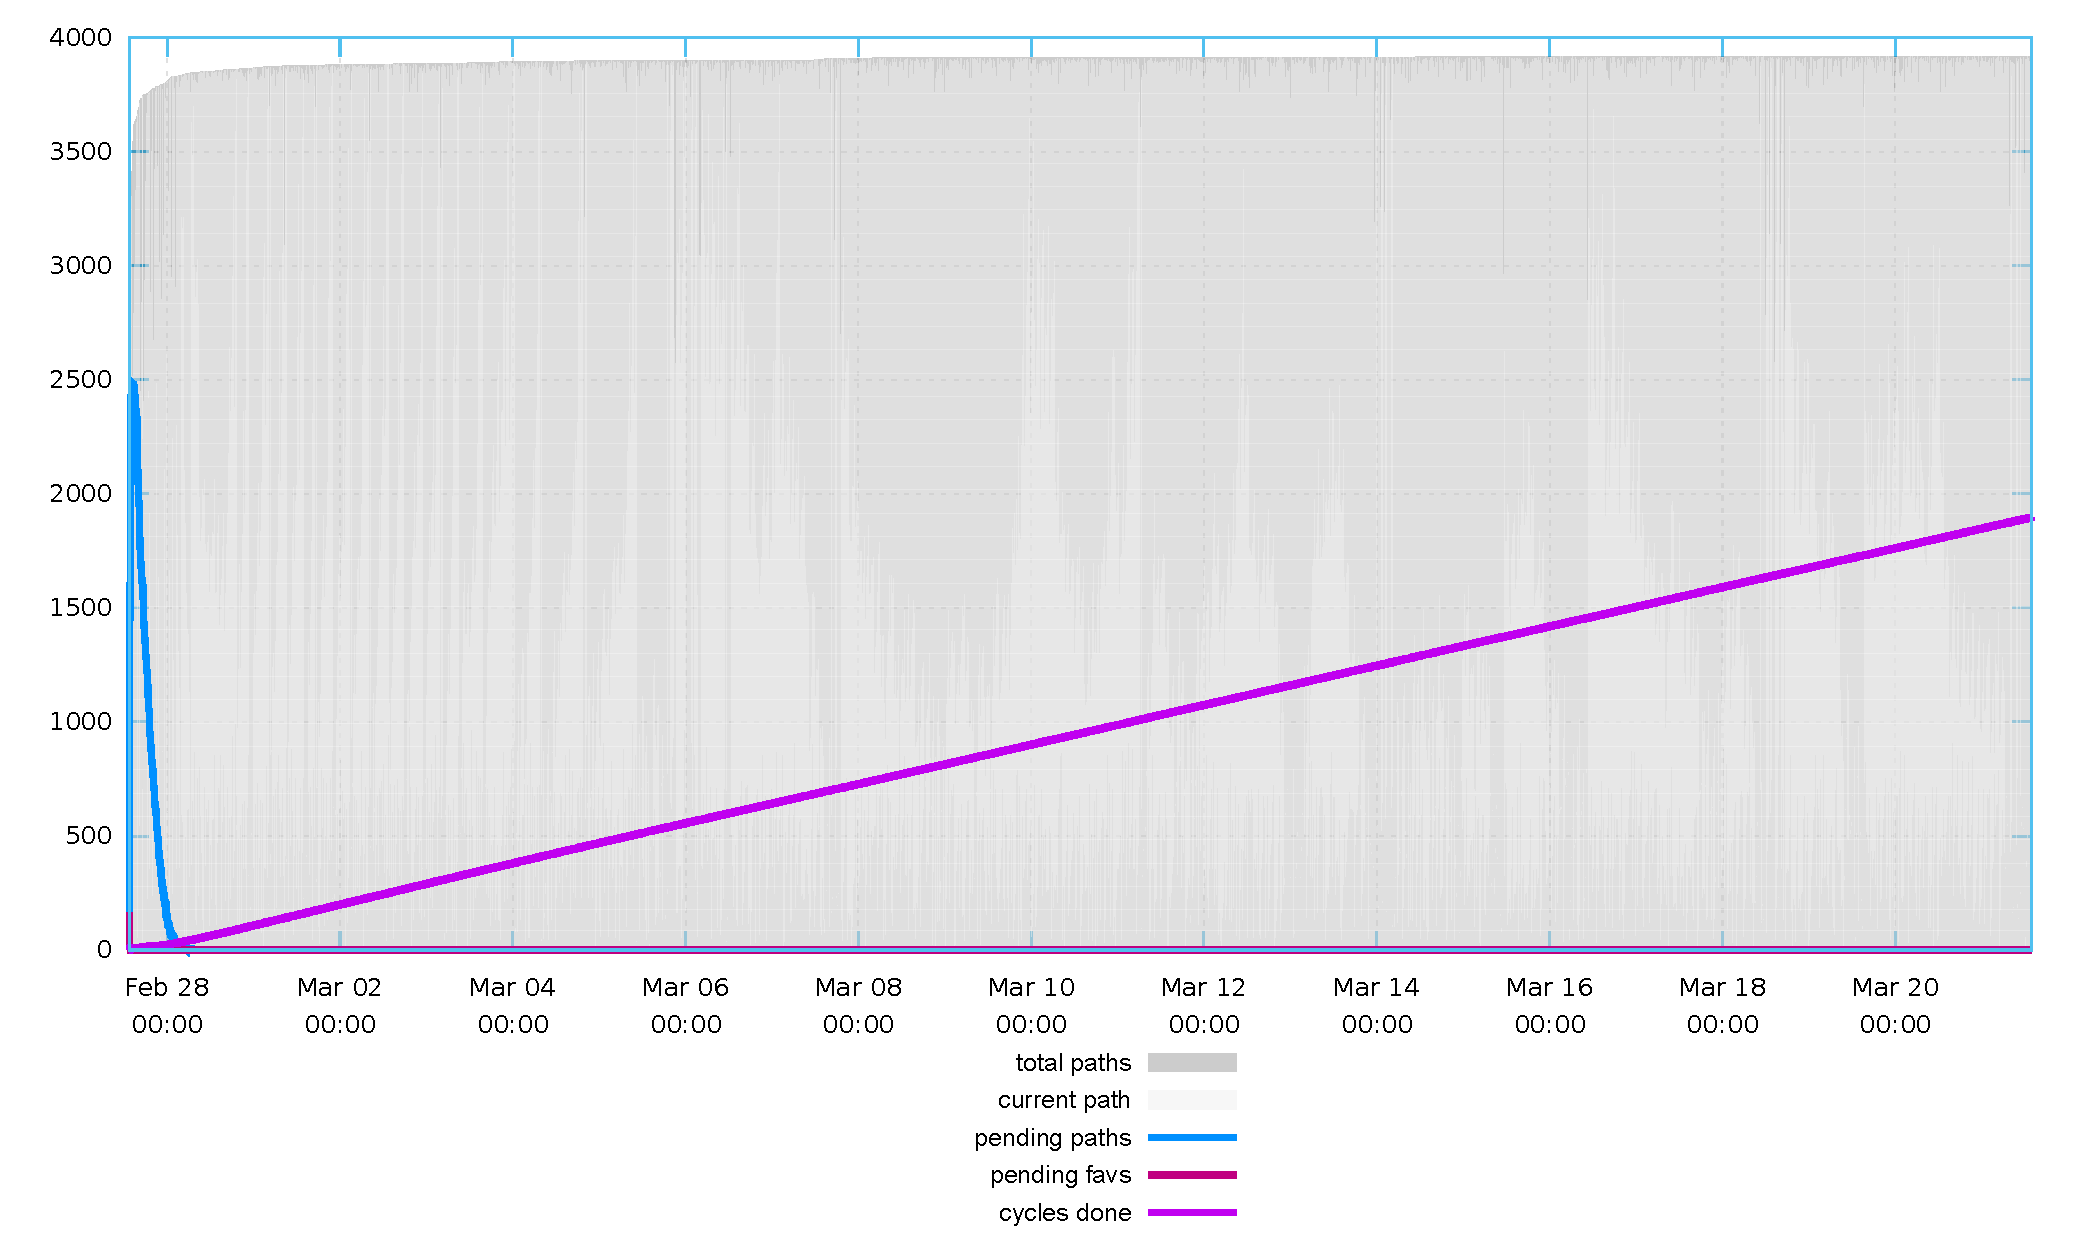
\includegraphics[width=\linewidth]{obrazky-figures/thread_1/high_freq.pdf}
	\caption{thread\_1/high\_freq}
	\label{fuz:result2b}
\end{figure}

\begin{figure}[H]
	\centering
	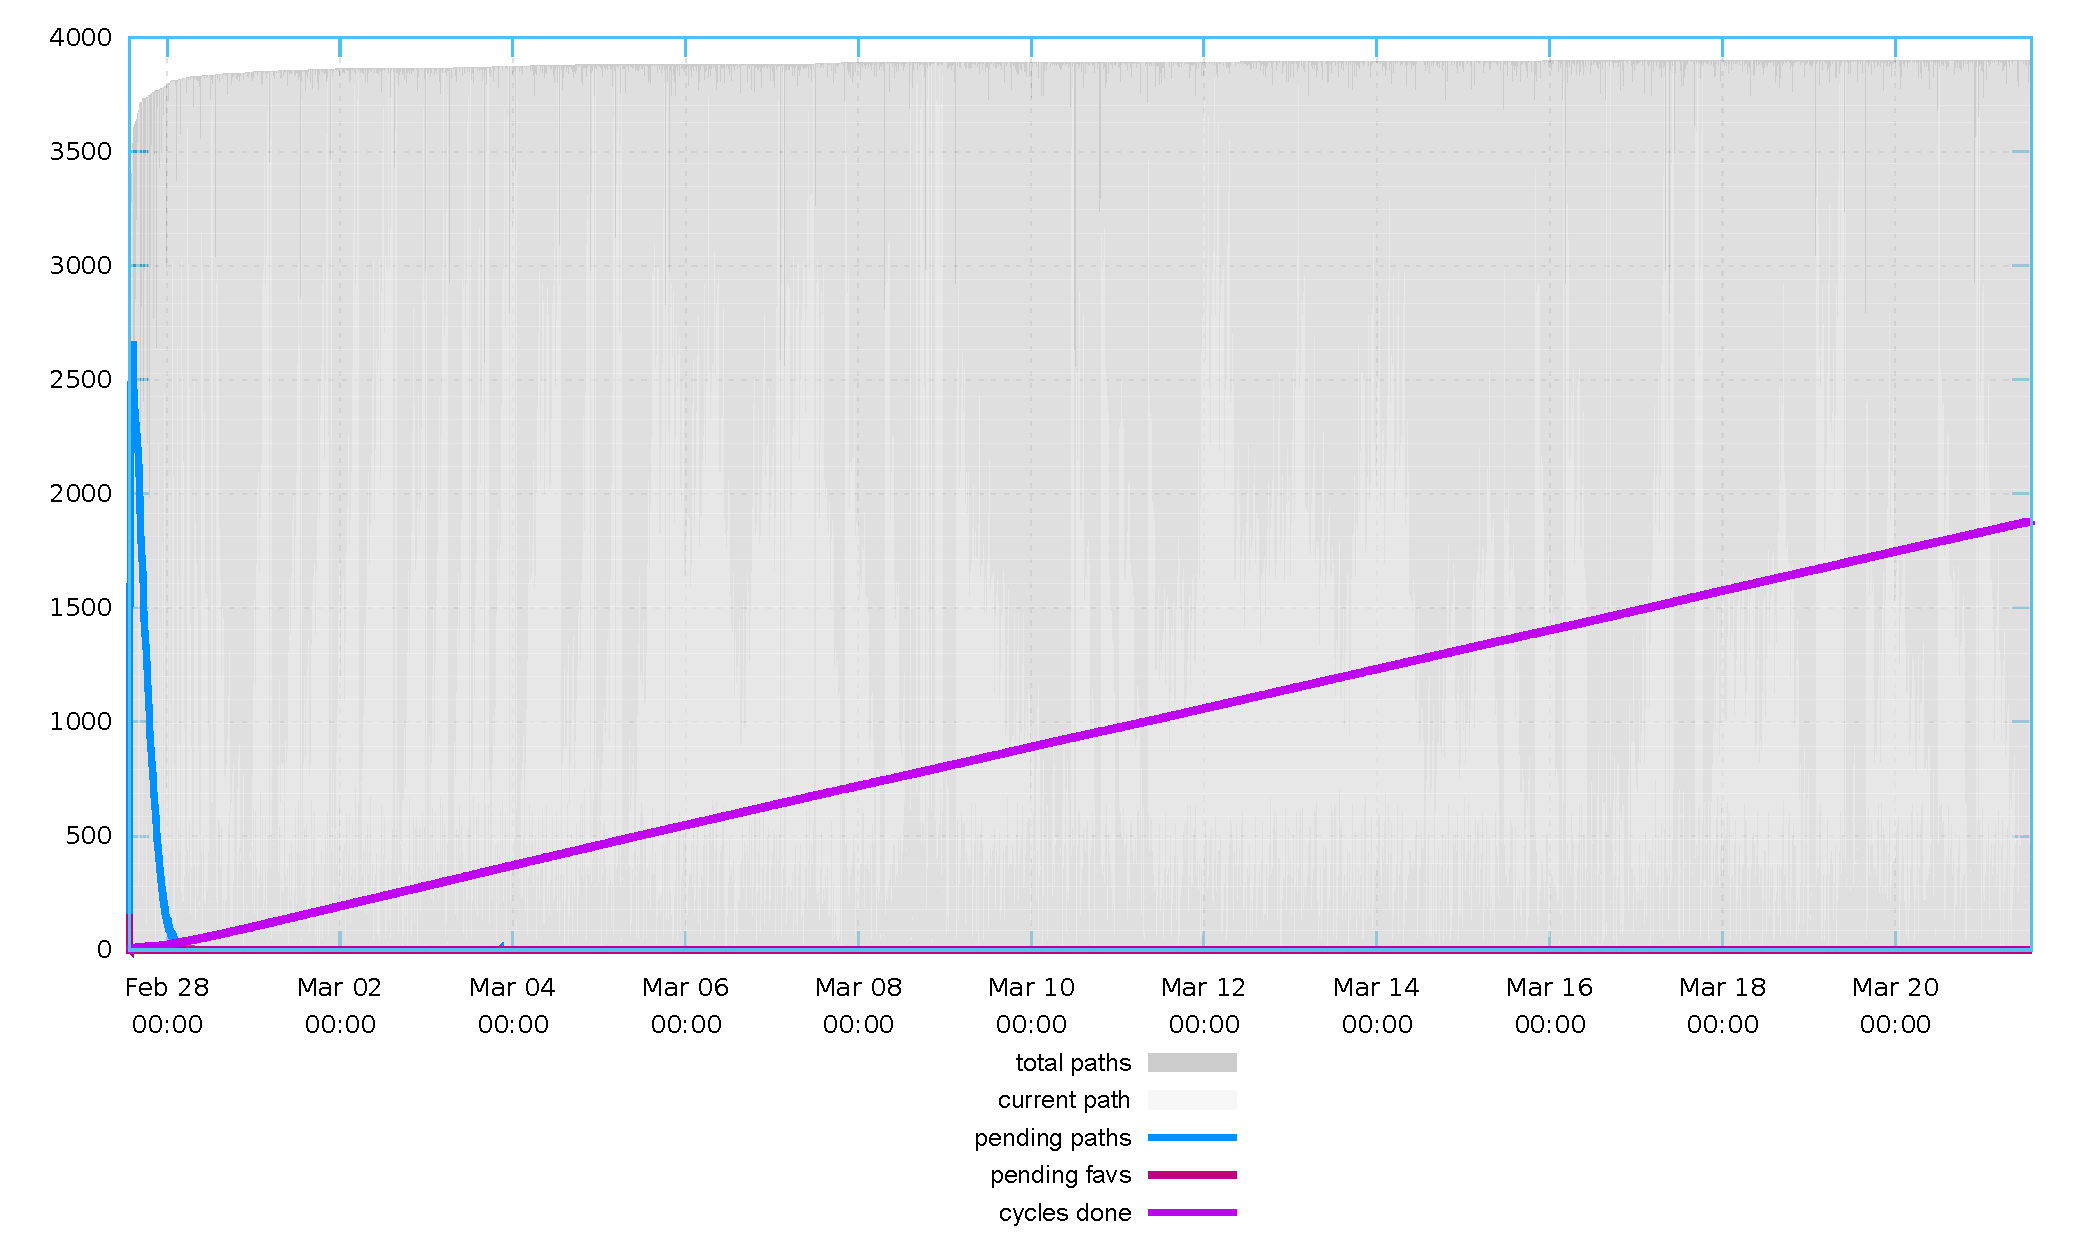
\includegraphics[width=\linewidth]{obrazky-figures/thread_2/high_freq.pdf}
	\caption{thread\_2/high\_freq}
	\label{fuz:result3b}
\end{figure}

\begin{figure}[H]
	\centering
	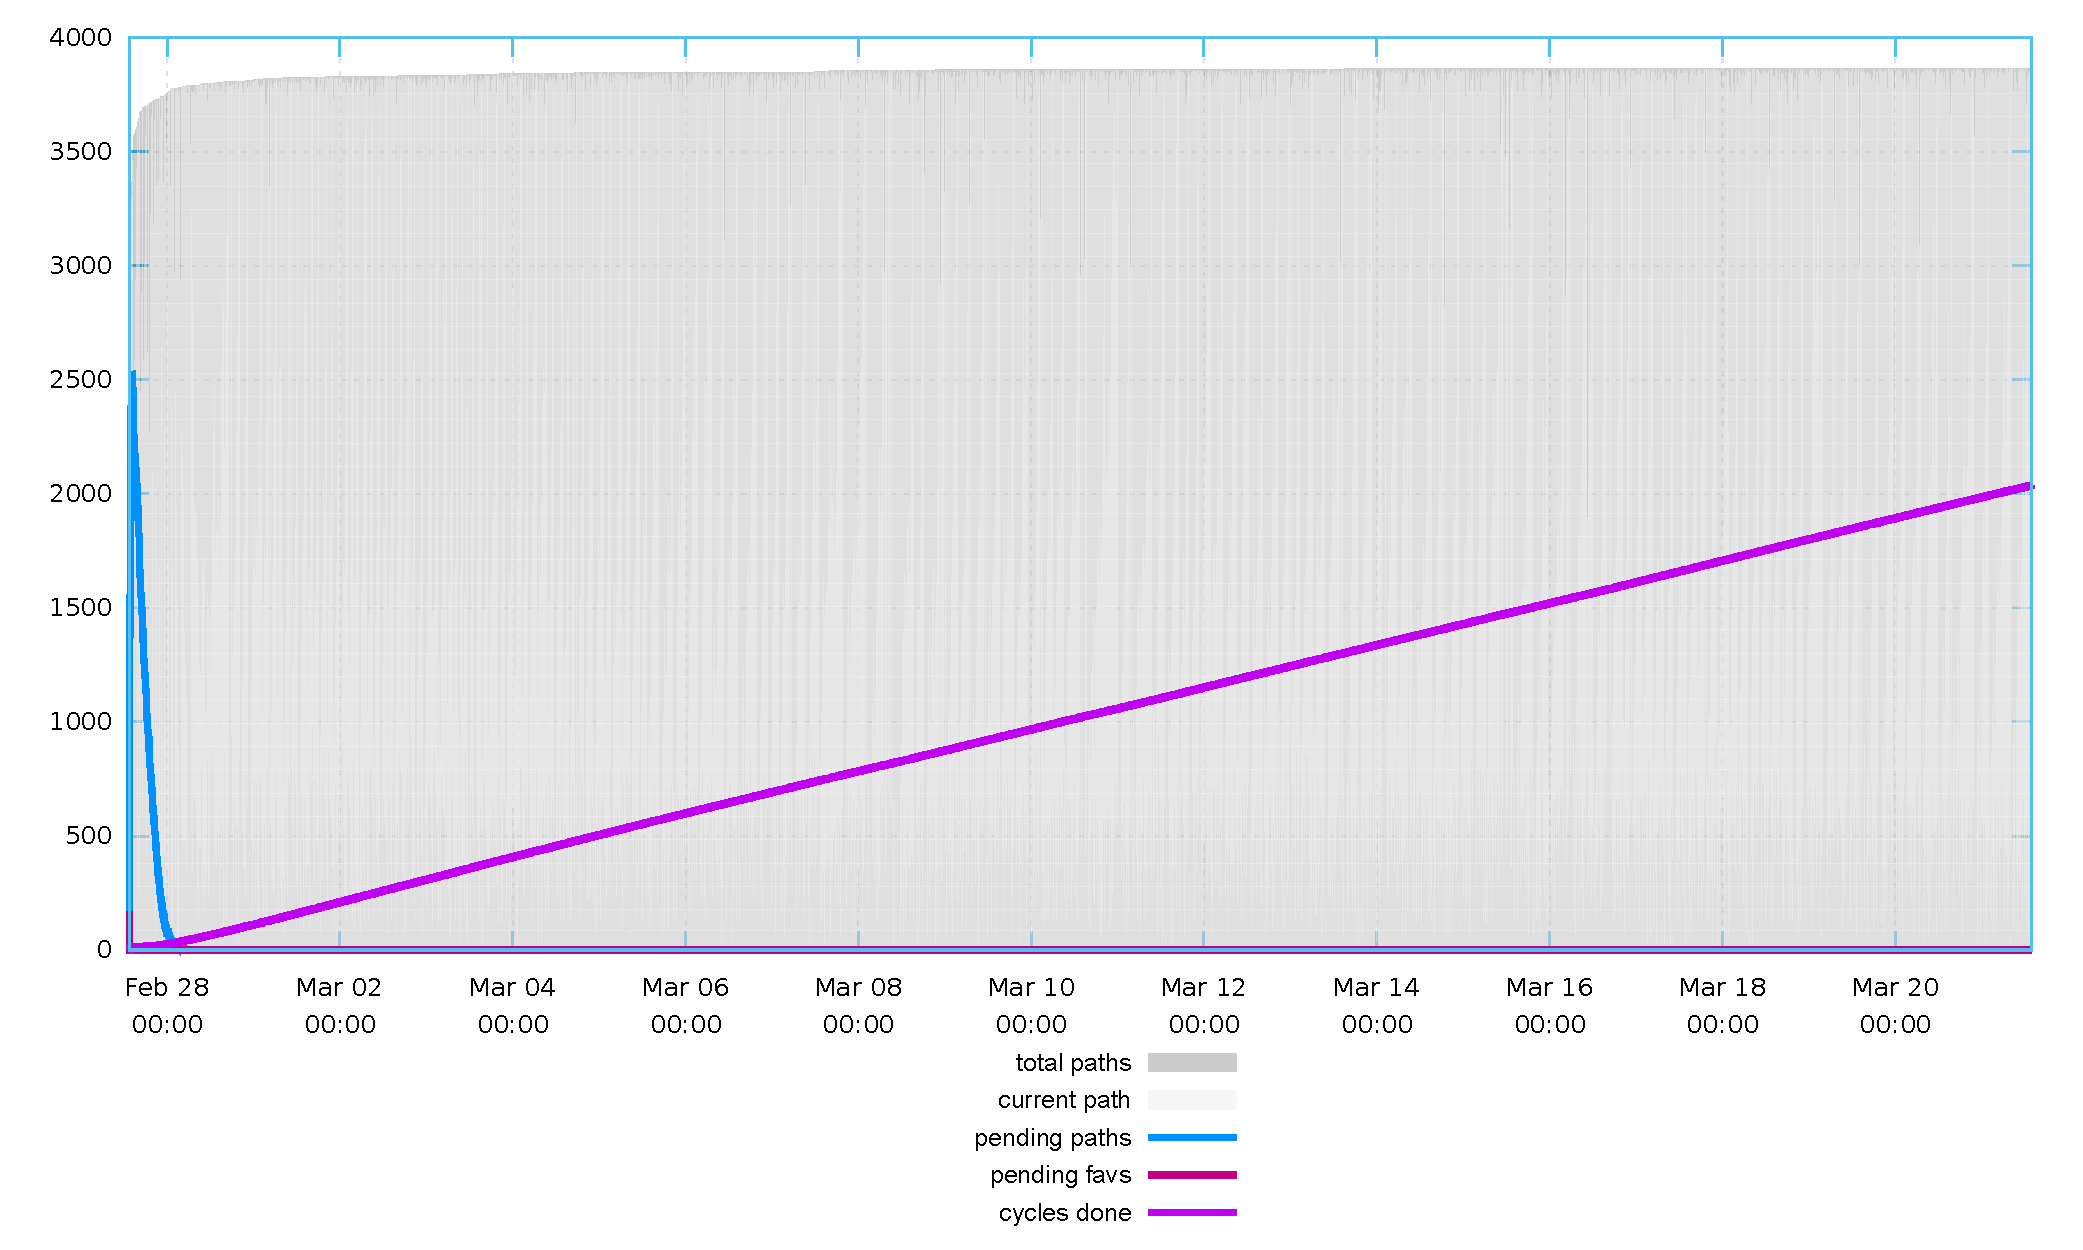
\includegraphics[width=\linewidth]{obrazky-figures/thread_3/high_freq.pdf}
	\caption{thread\_3/high\_freq}
	\label{fuz:result4b}
\end{figure}

asdfasdfasfasdfasdfasfasdfasdfasfasdfasdfasf

\begin{figure}[H]
	\centering
	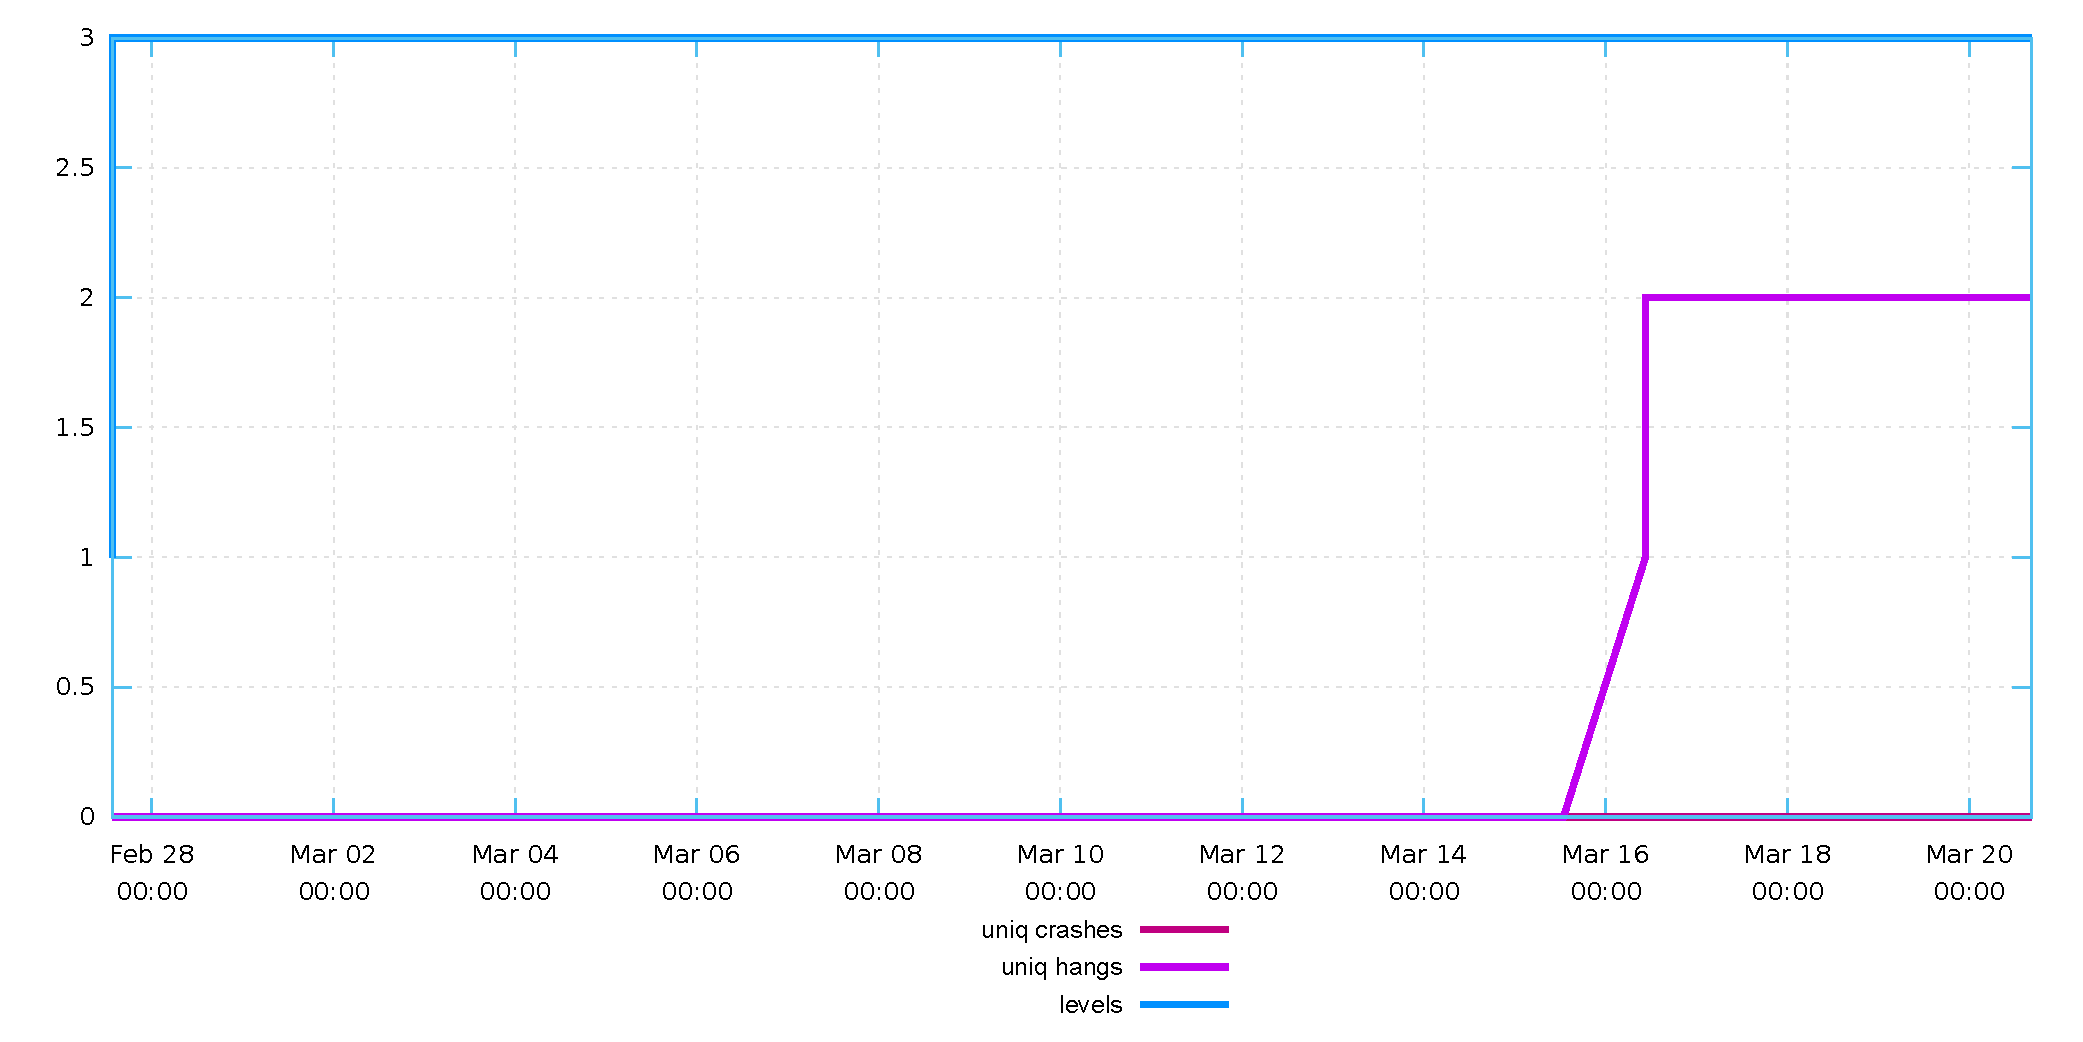
\includegraphics[width=\linewidth]{obrazky-figures/master/low_freq.pdf}
	\caption{master/low\_freq}
	\label{fuz:result1c}
\end{figure}

\begin{figure}[H]
	\centering
	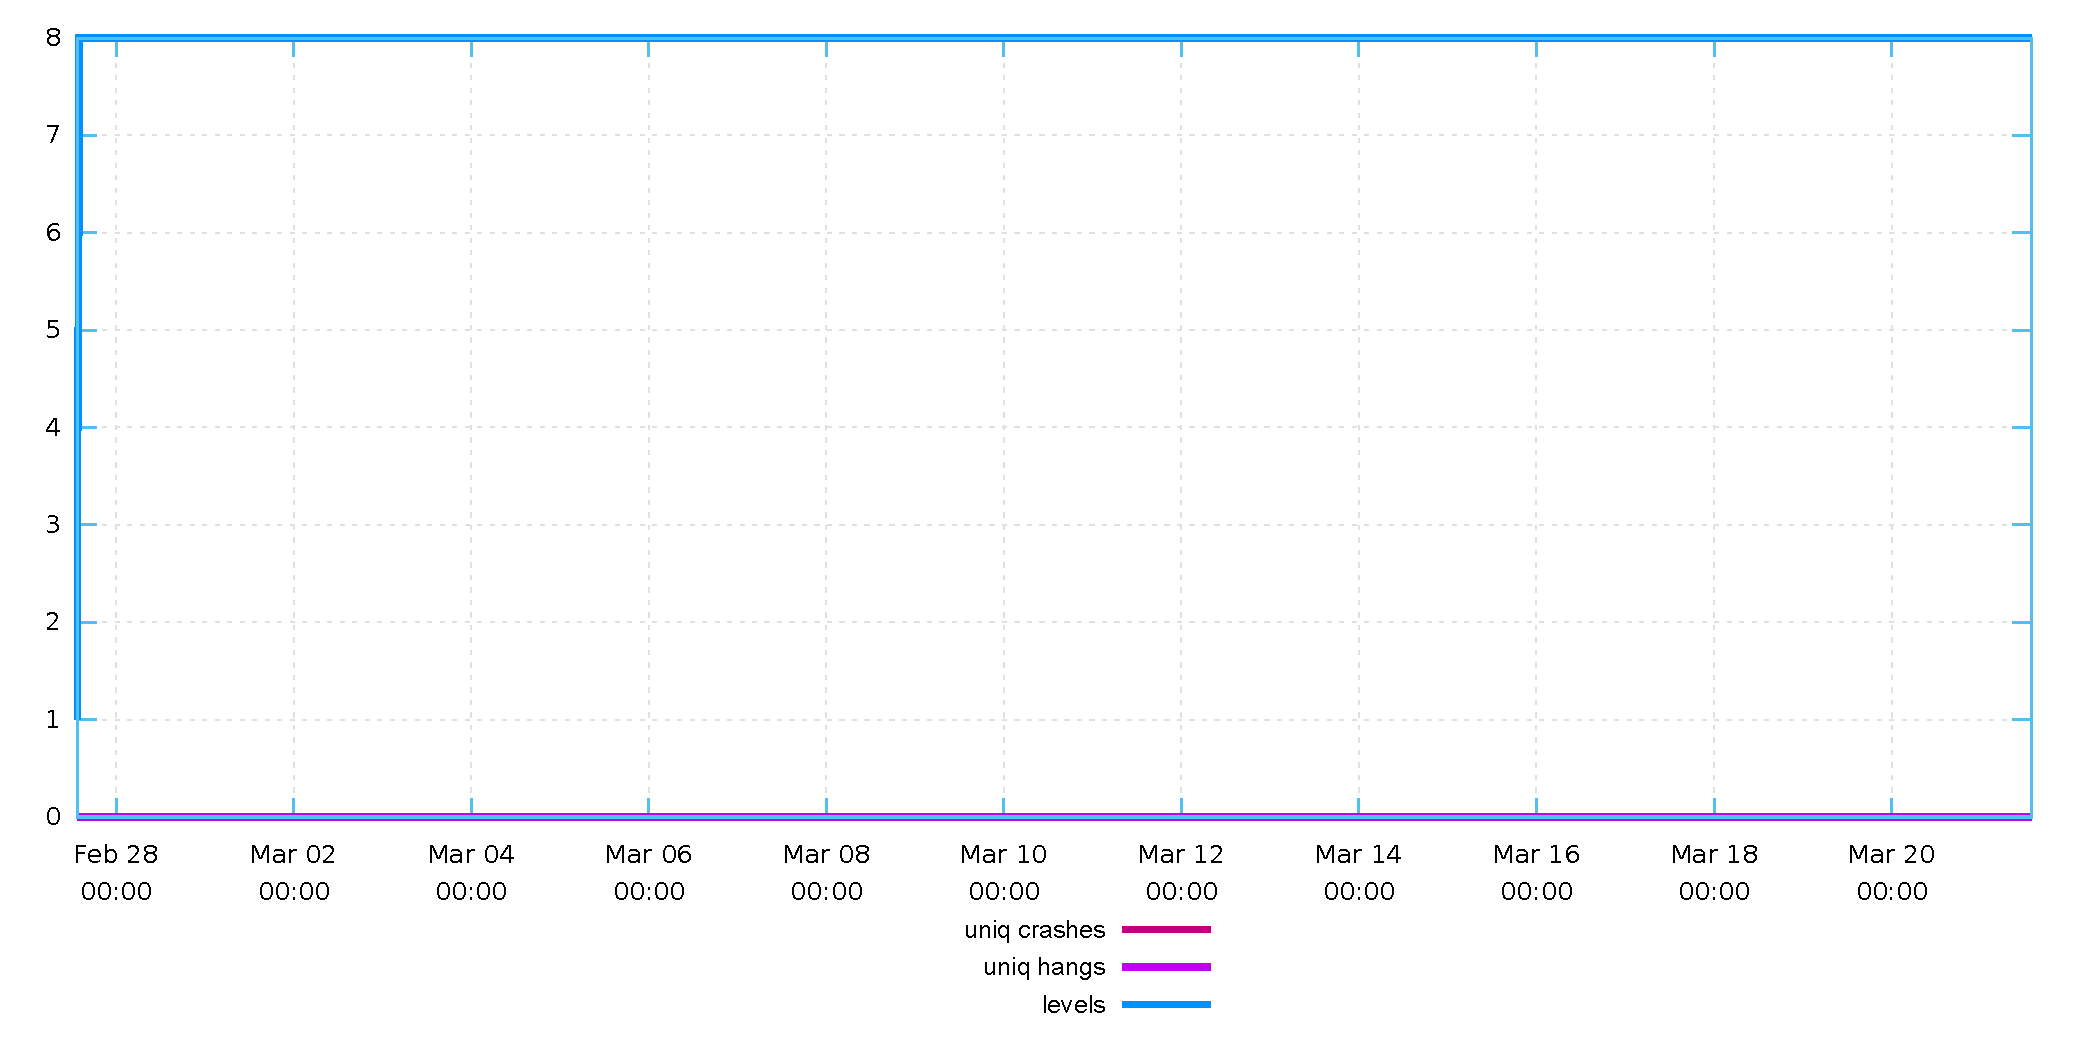
\includegraphics[width=\linewidth]{obrazky-figures/thread_1/low_freq.pdf}
	\caption{thread\_1/low\_freq}
	\label{fuz:result2c}
\end{figure}

\begin{figure}[H]
	\centering
	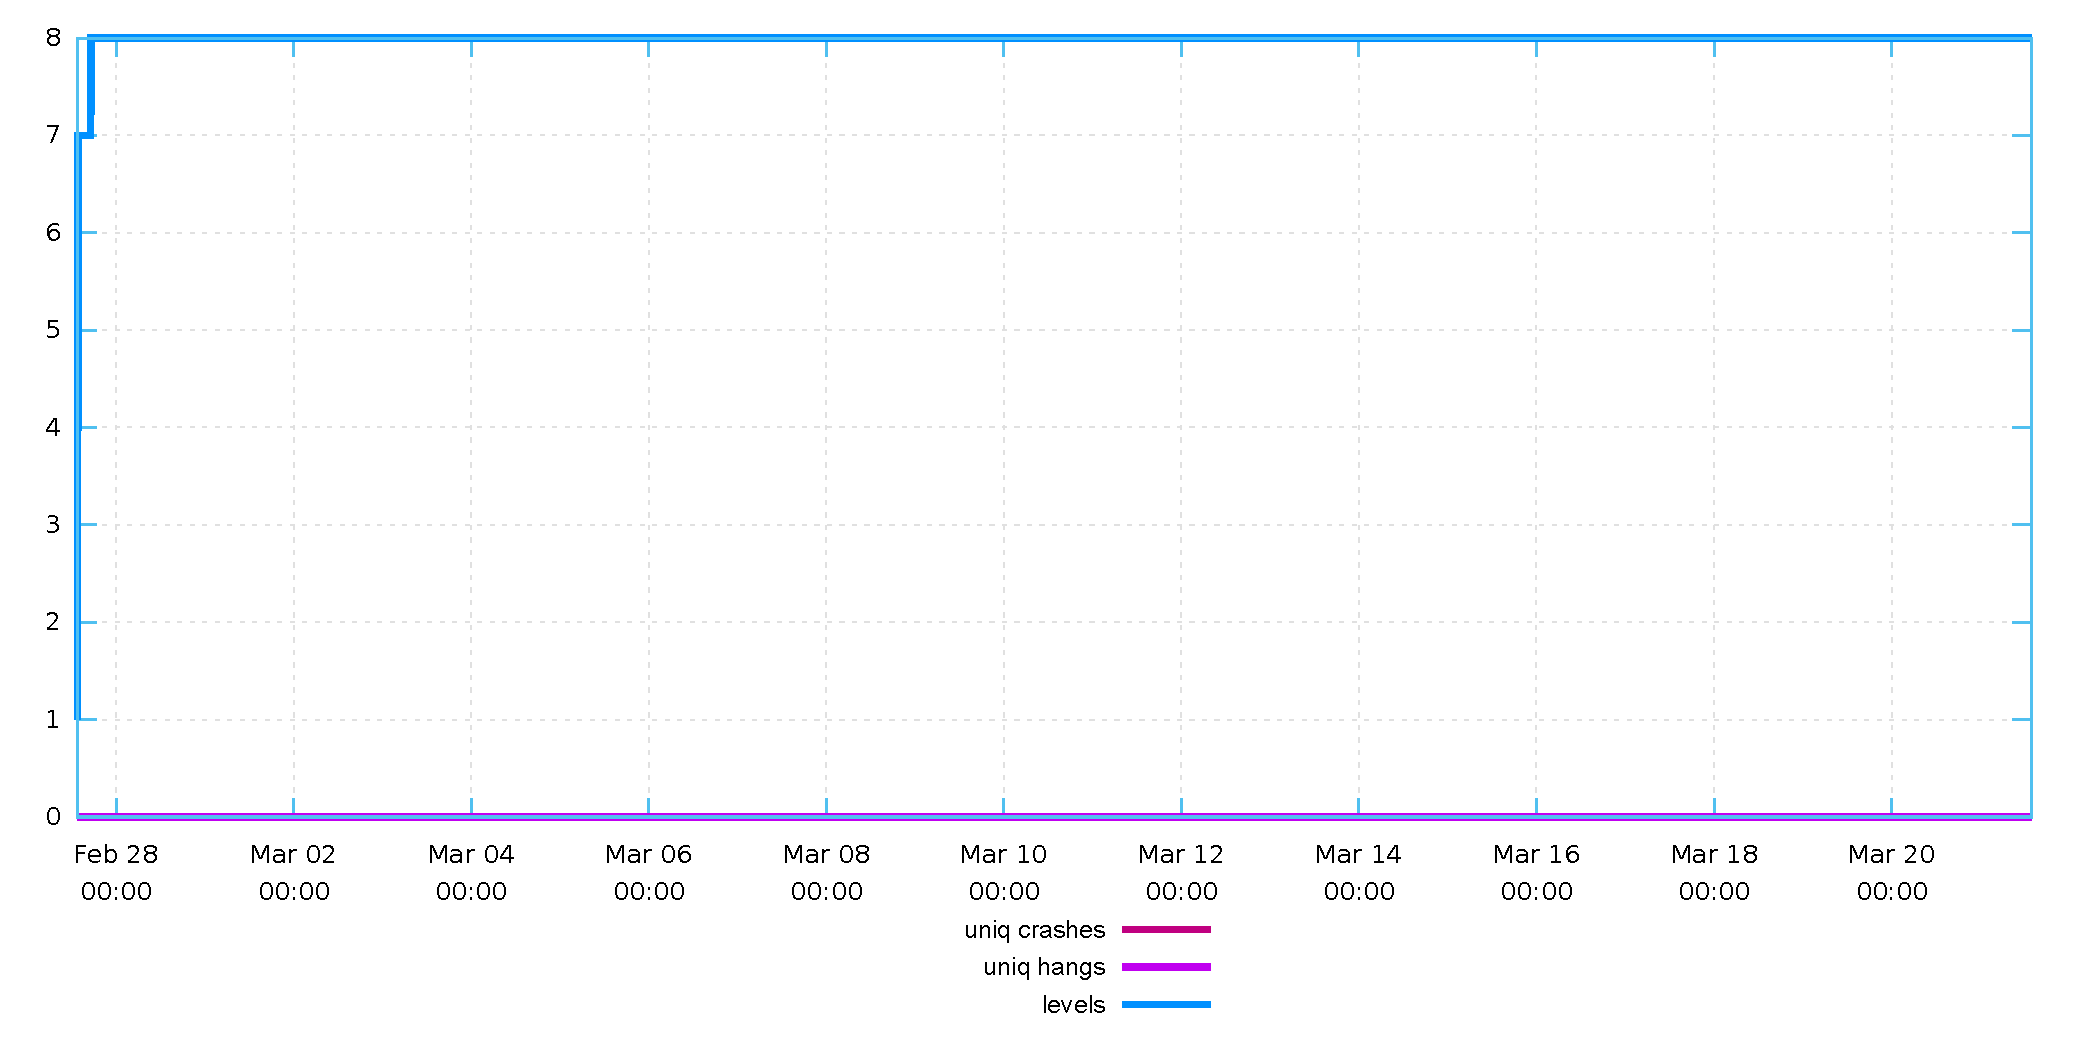
\includegraphics[width=\linewidth]{obrazky-figures/thread_2/low_freq.pdf}
	\caption{thread\_2/low\_freq}
	\label{fuz:result3c}
\end{figure}

\begin{figure}[H]
	\centering
	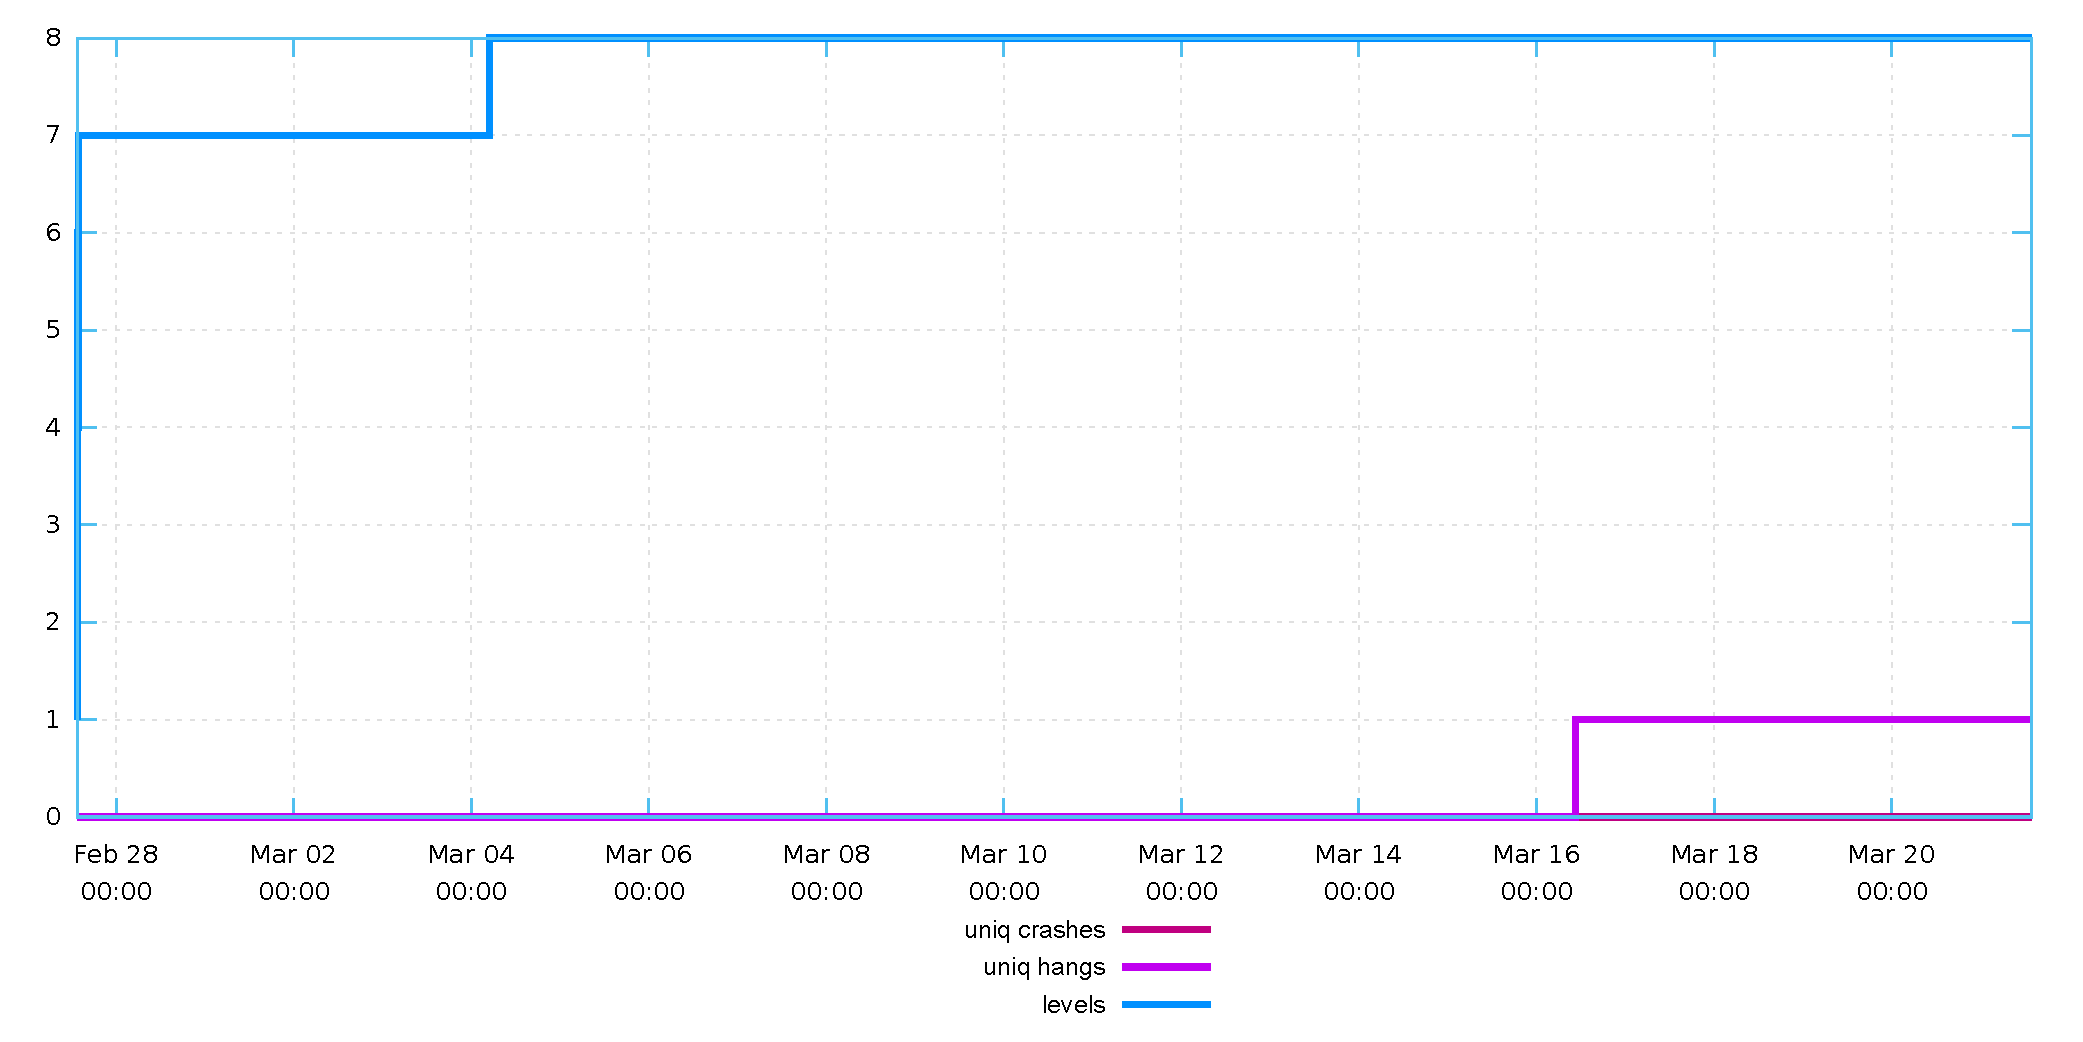
\includegraphics[width=\linewidth]{obrazky-figures/thread_3/low_freq.pdf}
	\caption{thread\_3/low\_freq}
	\label{fuz:result4c}
\end{figure}

asdfasdfasfasdfasdfasfasdfasdfasfasdfasdfasfasdfasdfasf

\subsection{Algorithms}
How should we test the algorithms?

\subsection{Policy generator}
how should we test this adapter?

\section{System and Acceptance Testing}
In the book of ''Software Acceptance Testing'' is acceptance testing defined as:
\emph{''Acceptance testing is the formal testing activity that presents the product to the
customer by enterprise (many times it includes stakeholders as well).
This activity represents demonstration of a software product and shows to the customer
that the requirements fulfilled its obligations. By this activity you can decide if
the product is ready for deployment. The software items must be examined
to ensure that the provided product is complete i.e. the architecture must be audited to check if
it accurate reflects the software configuration. The test results are audited by functional
configuration audit to certify that the software product satisfies its specification etc.''} \cite{Schmidt2013335}

In this case the acceptance testing means \todo{todo}

\subsection{Testing on real app}
\subsection{USBGuard}

\section{Static analysis}
Any bugs?

\section{Test Requirements}

\section{Results}
Which bugs have you found.

\chapter{Conclusion}



%=========================================================================


  % Kompilace po částech (viz výše, nutno odkomentovat)
  % Compilation piecewise (see above, it is necessary to uncomment it)
  %\subfile{projekt-01-uvod-introduction}
  % ...
  %\subfile{chapters/projekt-05-conclusion}


  % Pouzita literatura / Bibliography
  % ----------------------------------------------
\ifslovak
  \makeatletter
  \def\@openbib@code{\addcontentsline{toc}{chapter}{Literatúra}}
  \makeatother
  \bibliographystyle{bib-styles/czechiso}
\else
  \ifczech
    \makeatletter
    \def\@openbib@code{\addcontentsline{toc}{chapter}{Literatura}}
    \makeatother
    \bibliographystyle{bib-styles/czechiso}
  \else
    \makeatletter
    \def\@openbib@code{\addcontentsline{toc}{chapter}{Bibliography}}
    \makeatother
    \bibliographystyle{bib-styles/englishiso}
  %  \bibliographystyle{alpha}
  \fi
\fi
  \begin{flushleft}
  \bibliography{xtamas01-20-literatura-bibliography}
  \end{flushleft}

  % vynechani stranky v oboustrannem rezimu
  % Skip the page in the two-sided mode
  \iftwoside
    \cleardoublepage
  \fi

  % Prilohy / Appendices
  % ---------------------------------------------
  \appendix
\ifczech
  \renewcommand{\appendixpagename}{Přílohy}
  \renewcommand{\appendixtocname}{Přílohy}
  \renewcommand{\appendixname}{Příloha}
\fi
\ifslovak
  \renewcommand{\appendixpagename}{Prílohy}
  \renewcommand{\appendixtocname}{Prílohy}
  \renewcommand{\appendixname}{Príloha}
\fi
%  \appendixpage

% vynechani stranky v oboustrannem rezimu
% Skip the page in the two-sided mode
%\iftwoside
%  \cleardoublepage
%\fi

\ifslovak
%  \section*{Zoznam príloh}
%  \addcontentsline{toc}{section}{Zoznam príloh}
\else
  \ifczech
%    \section*{Seznam příloh}
%    \addcontentsline{toc}{section}{Seznam příloh}
  \else
%    \section*{List of Appendices}
%    \addcontentsline{toc}{section}{List of Appendices}
  \fi
\fi
  \startcontents[chapters]
  \setlength{\parskip}{0pt}
  % seznam příloh / list of appendices
  % \printcontents[chapters]{l}{0}{\setcounter{tocdepth}{2}}

  \ifODSAZ
    \setlength{\parskip}{0.5\bigskipamount}
  \else
    \setlength{\parskip}{0pt}
  \fi

  % vynechani stranky v oboustrannem rezimu
  \iftwoside
    \cleardoublepage
  \fi

  % Přílohy / Appendices
  \chapter{Comparison of libseccomp and raw BPF filtering}

\section{BPF}
\lstinputlisting[language=c, label={lst:raw_bpf}, caption={Using raw BPF filtering}]{source_examples/raw_bpf.c}

\section{libseccomp}
\lstinputlisting[language=c, label={lst:libseccomp}, caption={Using simpler libseccomp wrapper}]{source_examples/libseccomp.c}

\chapter{Output of strace2seccomp}

\section{Example Output no.1}
\lstinputlisting[language=c, label={lst:example1}, caption={Example output of strace2seccomp}]{source_examples/exportedSource.c}


  % Kompilace po částech (viz výše, nutno odkomentovat)
  % Compilation piecewise (see above, it is necessary to uncomment it)
  %\subfile{xtamas01-30-prilohy-appendices}

\end{document}
